\documentclass[12pt, oneside, letterpaper]{amsbook}

%a continuaci?n el paquete que permite incluir gr?ficos
\usepackage{graphics}

%el siguiente paquete permite acentuar de la manera usual
%se recomienda usarlo porque facilita la correcci?n de la tesis
%con un diccionario de espa?ol
\usepackage[ansinew]{inputenc}
%\usepackage[utf8]{inputenc}

%a continuaci?n el paquete y el comando para que las figuras no se
%ubiquen siempre en la parte de arriba de la p?gina
\usepackage{float}
\floatplacement{figure}{ht}

%el uso del siguiente paquete (babel) va a permitir que las palabras
%se separen correctamente
%no olvide seleccionar "spanish" al principio del documento
\usepackage[spanish,english]{babel}


%el siguiente comando permite la elaboraci?n del ?ndice anal?tico
\makeindex

%el siguiente grupo de comandos fija los m?rgenes del documento

% Set left margin - The default is 1 inch, so the following
\setlength{\oddsidemargin}{0in}
%\setlength{\evensidemargin}{-0.1in}

% Set width of the text - What is left will be the right margin.
\setlength{\textwidth}{6.5in}

% Set top margin - The default is 1 inch, so the following
% command sets a 0.75-inch top margin.
\setlength{\topmargin}{-.4in}

% Set height of the text - What is left will be the bottom margin.
% In this case, bottom margin is 11in - 0.75in - 9.5in = 0.75in
\setlength{\textheight}{9in}

% Set height of the header
%\setlength{\headheight}{0.3in}

% Set vertical distance between the header and the text
\setlength{\headsep}{0.4in}

% Set vertical distance between the text and the
% bottom of footer
\setlength{\footskip}{0.4in}

%el siguiente comando define el espacio entre lineas
\renewcommand{\baselinestretch}{1.5}

%los siguientes comando cambian los nombres "Chapter", "Proof", etc
%a "Cap?tulo", "Demostraci?n", etc.
%NO hacen falta si usa el paquete "babel"

\renewcommand{\chaptername}{Cap\'{\i}tulo}
\renewcommand{\contentsname}{CONTENIDO}
\renewcommand{\proofname}{Demostraci\'on}
\renewcommand{\bibname}{Bibliograf\'{\i}a}
\renewcommand{\indexname}{\'Indice}
\renewcommand{\figurename}{Figura}

%el siguiente comando define "seno" como funci?n (esta funci?n
%no la trae LaTeX porque es ingl?s es "sine")
%igual para arcoseno
\newcommand{\sen}{\operatorname{sen}}
\newcommand{\arcsen}{\operatorname{arcsen}}

\theoremstyle{plain}
\newtheorem{theorem}{Teorema}[chapter]
\newtheorem{proposition}[theorem]{Proposici\'on}
\newtheorem{lemma}[theorem]{Lema}
\newtheorem{corollary}[theorem]{Corolario}


\theoremstyle{definition}
\newtheorem{definition}[theorem]{Definici\'on}
\newtheorem{example}[theorem]{Ejemplo}



\theoremstyle{remark}
\newtheorem{remark}[theorem]{Observaci\'on}

\numberwithin{equation}{chapter} \numberwithin{figure}{chapter}


%Optativo
%el siguiente paquete hace que el documento tenga hiperv?nculos
%es muy ?til a la hora de tipear y hace la versi?n electr?nica
%mucho m?s atractiva
%se debe colocar justo antes de "\begin{document}"

%\usepackage[letterpaper,backref,plainpages=false,pagebackref]{hyperref}


\begin{document}

\selectlanguage{spanish}

\frontmatter


\thispagestyle{empty}


\begin{center}

\vspace*{-1.5cm}

\scalebox{.12}{
\includegraphics{ucv.eps}}

\vspace{.5cm}

\begin{small}
UNIVERSIDAD CENTRAL DE VENEZUELA

\vspace{-0.1cm}

FACULTAD DE CIENCIAS

\vspace{-0.1cm}

ESCUELA DE MATEM\'ATICA

\vspace{-0.1cm}

MAESTR\'IA EN MODELOS ALEATORIOS

\vspace{-0.1cm}

\end{small}

\vspace{2cm}

\begin{Huge}

{\bf Estimaci\'on de la curva de rendimientos mediante}

{\bf el uso de splines c\'ubicos suavizados}


\end{Huge}

\end{center}

\vspace{2cm}

\hspace{6cm}
\begin{minipage}[t]{9cm}
%\begin{large}
Trabajo de Grado de Maestr\'ia presentado ante la ilustre Universidad Central de Venezuela por el
\textbf{Lic. Freddy F. Tapia C.} para optar al t\'{\i}tulo de \textbf{Magister Scientiarium Menci\'on Modelos Aleatorios}

\

\textbf{Tutor: Dr. Ricardo Rios.}
%\end{large}
\end{minipage}



\vspace{1.5cm}

\begin{center}
Caracas, Venezuela \\
Noviembre y 2018
\end{center}

\newpage


%%%%NO USAR EN TESIS DE POSTGRADO%%%%%%%%


Nosotros, los abajo firmantes, designados por la Universidad Central de Venezuela como
integrantes del Jurado Examinador del Trabajo Especial de Grado titulado ``\textbf{Nombre del
Trabajo Especial de Grado}'', presentado por el \textbf{Br. Nombre del Estudiante}, titular de
la C\'edula de Identidad \textbf{XXXXXXXXX}, certificamos que este trabajo cumple con los
requisitos exigidos por nuestra Magna Casa de Estudios para optar al t\'{\i}tulo de
\textbf{Licenciado en Matem\'atica}.

%%%%NO USAR EN TESIS DE POSTGRADO%%%%%%%%


\vspace{2cm}

\begin{center}
\underline{\hspace{8cm}}

\vspace{1cm}

\textbf{ Nombre del Tutor \\Tutor}

\vspace{3cm}

\underline{\hspace{8cm}}

\vspace{1cm}

\textbf{ Nombre del Jurado \\Jurado}

\vspace{3cm}

\underline{\hspace{8cm}}

\vspace{1cm}

\textbf{ Nombre del Jurado \\Jurado}

\end{center}

\newpage


\vspace*{2.5cm}

\begin{center}
{\large Dedicatoria}
\end{center}
\vspace{1cm}

Colocar aqu\'{\i} la dedicatoria (optativo).

\newpage


\vspace*{2.5cm}

\begin{center}
{\large Agradecimiento}
\end{center}
\vspace{1cm}

Colocar aqu\'{\i} el agradecimiento (optativo).

\newpage



\tableofcontents


\mainmatter

\chapter*{Introducci\'on.}

\hspace*{0.4 cm} La curva de redimientos es una herramienta ampliamente utilizada por las autoridades de los bancos centrales en sus decisiones de pol\'itica monetaria, as\'i como tambi\'en por los agentes privados en la planificaci\'on de sus inversiones en instrumentos financieros [1]. La misma tiene una importancia capital
para el mundo acad\'emico y pr\'actico desde el punto de vista econ\'omico y financiero, al reflejar el precio intertemporal del dinero.


\hspace*{0.4 cm} Uno de los principales objetivos que se persigue mediante el uso de esta herramienta, es el de estimar los precios de los t\'itulos de la deuda p\'ublica nacional que posee una instituci\'on financiera en su portafolio de inversiones en un per\'iodo determinado. Para ello es importante conocer las caracter\'isticas de los t\'itulos \'o instrumentos que existen en el mercado venezolano, entre ellos tenemos los siguientes,


\begin{itemize}
  \item T\'itulos de inter\'es fijo (TIF): son instrumentos que se caracterizan por tener una renta fija, y se emiten en moneda nacional.
  \item T\'itulos de inter\'es variable (VEBONO): se caracterizan por poseer una renta variable, e igual que los TIF se emiten en Bol\'ivares.
  \item Bonos PDVSA : son instrumentos emitidos en d\'olares.
\end{itemize}


\hspace*{0.4 cm}Cabe destacar que en el presente trabajo s\'olo  se considerar\'an aquellos instrumentos emitidos en Bol\'ivares.


\hspace*{0.4 cm}Asociado a cada t\'itulo hay un monto de dinero que se invierte, el cual es entregado al ente emisor por el t\'itulo en s\'i, existe tambi\'en una fecha de emisi\'on, y una fecha de vencimiento, d\'ia en el cual el ente emisor retorna el monto invertido inicialmente. Es importante destacar que estos t\'itulos pagan un inter\'es al portador cada tres meses, y esta representa la ganancia que tiene el inversionista.


\hspace*{0.4 cm} Con el fin de determinar en que t\'itulo es mejor invertir, es necesario conocer el rendimiento al vencimiento que posee dicho t\'itulo, este valor nos da un idea de cu\'al ser\'a el retorno que recibir\'a el portador del t\'itulo por la tenencia o compra del mismo. Para calcular este valor es necesario conocer la fecha de vencimiento del t\'itulo as\'i como su valor nominal y su precio.


 \hspace*{0.4 cm} A partir de la siguiente f\'ormula podemos hallar dicho valor,

\vspace{0.5cm}

\begin{center}

$\displaystyle{P_{t,m} = \sum_{i=1}^{m-1}{\frac{c}{(1+R_{t,i})^i} + \frac{1+c}{(1+R_{t,m})^m}}, }$

\end{center}

\vspace{0.5cm}

\noindent donde $P_{t,m}$ representa el precio del t\'itulo al tiempo t, y que tiene un vencimiento de m a\~nos, c representa el cup\'on asociado al t\'itulo, el \'indice $i = 1,...,m$ representa cuantos cupones todav\'ia le quedan al t\'itulo por pagar antes de su vencimiento. Por su parte $R_{t,m}$ representa el rendimiento al vencimiento del t\'itulo en el tiempo t y que tiene un vencimiento de m a\~nos.


\hspace*{0.4 cm}A partir de la f\'ormula anterior podemos afirmar que para calcular el rendimiento al vencimiento de un t\'itulo es necesario conocer su precio a una fecha espec\'ifica, pero esto no siempre es posible, esto se debe a las caracter\'isticas del mercado venezolano ya que son pocos los t\'itulos que cotizan y por ende no se conoce su precio.


\hspace*{0.4 cm} Dicho precio puede conocerse a diario mediante la informaci\'on suministrada en la pesta\~na ``0-22" del documento ``resumersec" del Banco Central de Venezuela, este ente publica cada d\'ia las operaciones realizadas con estos instrumentos, en este documento se puede obtener el precio de aquellos t\'itulos que coticen ese d\'ia, el problema radica en conocer los precios de aquellos t\'itulos que no est\'en en dicho documento.



\hspace*{0.4 cm} La curva de rendimientos presenta emp\'iricamente una serie de dificultades, debido a que se construye a trav\'es de una serie de precios (tasas) de instrumentos financieros discontinuos en el tiempo que, por lo general, est\'an lejos de ser una curva suave. Para su estimaci\'on existen diversas metodolog\'ias, las param\'etricas y las no param\'etricas.


\hspace*{0.4 cm} Las metodolog\'ias param\'etricas se basan en modelos asociados a una familia funcional que
obedece al comportamiento de alguna distribuci\'on de probabilidad, sobre la cual suponemos que las caracter\'isticas de la poblaci\'on de inter\'es pueden ser descritas. Es as\'i como, los modelos dise\~nados en este contexto, basados en regresi\'on, buscan describir el comportamiento de una variable de inter\'es con otras llamadas ex\'ogenas, a trav\'es de funciones de v\'inculo lineales o no lineales.


\hspace*{0.4 cm}Entre estas metodolog\'ias destacan, la de Nelson y Siegel introducida en $1987$ [2], la de Svesson desarrollada en $1994$ [3], la metodolog\'ia de los polinomios por componentes principales propuesta por Hunt y Terry en $1998$ [4], as\'i como los polinomios trigonom\'etricos desarrollada por Nocedal y Wright en $1999$ [5].


\hspace*{0.4 cm} Por su parte, las metodolog\'ias no param\'etricas se han convertido en los \'ultimos a\~nos en un
\'area de gran estudio debido a sus ventajas relativas respecto a los modelos de regresi\'on basado en funciones. Entre las caracter\'isticas m\'as importantes de estos modelos tenemos, la flexibilidad en los supuestos y el ajuste dirigido espec\'ificamente a trav\'es de los datos. Entre estas metodolog\'ias se destacan la de regresi\'on Kernel, polinomios locales, splines de polinomios (Fan y Gibels, $1996$ [6]), splines c\'ubicos suavizados (B.W. Silverman, $1985$ [7]), super suavizador de Friedmann (Friedmann, $1984$ [8]) y redes neuronales artificiales (Sharda, $1994$ [9]).



\hspace*{0.4 cm} En el siguiente trabajo se propone el uso de la metodolog\'ia de splines c\'ubicos suavizados, la cual posee la ventaja de contar con un factor de penalizaci\'on el cu\'al es muy \'util al momento de tener un balance entre la suavidad de la curva y su bondad de ajuste. A grandes rasgos estas metodolog\'ias se basan en estimar la curva de rendimientos de dichos t\'itulos, curva que relaciona el rendimiento al vencimiento con la maduraci\'on o fecha de vencimiento, con el fin de estimar los precios de los t\'itulos a un d\'ia en espec\'ifico. De esta manera a partir de una determinada fecha es posible mediante estas metodolog\'ias estimar el rendimiento al vencimiento de un t\'itulo y por ende saber su precio estimado.


\hspace*{0.4 cm} La estructura del presente trabajo se presenta a continuaci\'on, en el cap\'itulo 1 se encuentran los antecendentes de trabajos anteriores y la motivaci\'on del mismo. En el cap\'itulo 2 se presenta toda la parte te\'orica que sustenta esta metodolog\'ia, as\'i como las herramientas necesarias para la implementaci\'on de la misma.

\hspace*{0.4 cm} En el cap\'itulo 3, se expone el marco metodol\'ogico, en esta parte se explica el proceso de la elaboraci\'on de la base de datos, su depuraci\'on para luego poder aplicar la metodolog\'ia de los Splines c\'ubicos de suavizado. Finalmente, en el cap\'itulo 4 se presentan los resultados y conclusiones que se obtuvieron luego de realizar el c\'alculo de los precios te\'oricos mediante diferentes metodolog\'ias.





\chapter{Antecedentes y motivaci\'on.}

% \hspace*{0.4 cm} La curva de redimientos es una herramienta ampliamente utilizada por las autoridades de los bancos centrales en sus decisiones de pol\'itica monetaria, as\'i como tambi\'en por los agentes privados en la planificaci\'on de sus inversiones en instrumentos financieros [1]. La misma tiene una importancia capital
% para el mundo acad\'emico y pr\'actico desde el punto de vista econ\'omico y financiero, al reflejar el precio intertemporal del dinero.

\section{Rendimiento.}

\hspace*{0.4 cm} El rendimiento es un t\'ermino utilizado en finanzas, bancos, t\'itulos y valores financieros, es el producto o utilidad que se obtiene de algo  de alguna inversi\'on. Es frecuente en \'epocas de inflaci\'on, que los intereses que otorguen otros instrumentos de inversi\'on, sean superiores a los que otorgan los bonos y obligaciones que llevan varios a\~nos de haberse emitido, lo cual resta inter\'es a la adquisici\'on de dichos bonos a menos que se les descuente en su precio la cantidad necesaria para hacerlos competitivos.

\hspace*{0.4 cm}Es as\'i como empiezan a operar los bonos y las obligaciones, ``con descuento", o ``abajo de su valor nominal". Quien compra un bono u obligaci\'on ``abajo de su valor nominal", espera recibir un inter\'es atractivo y, adicionalmente, una ganancia de capital en el momento en que venda el bono.

\hspace*{0.4 cm}El bono u obligaci\'on ir\'a subiendo de precio, hasta que llega a coincidir con el valor nominal, el d\'ia de su vencimiento. Es frecuente que los bonos y obligaciones no lleguen al vencimiento al $100\%$ el mismo d\'ia, sino que tengan amortizaciones previas (predefinidas) por sorteo o por serie. En estos casos, hay que emplear f\'ormulas especiales para llegar al rendimiento y vencimiento incluyendo las amortizaciones.

\subsection{Tipos de rendimiento.\\}

\hspace*{0.4 cm} En base al precio vigente, un bono muestra tres diferentes tipos de vencimiento,

\begin{itemize}
  \item El rendimiento del cup\'on es la tasa de inter\'es que paga el bono por su valor nominal. Un bono de $US\$10.000$ con un cup\'on del 6 por ciento de inter\'es paga $US\$300$ de inter\'es cada 6 meses.
  \item El rendimiento actual es la tasa del cup\'on dividida por el precio del bono. Si el bono con un valor nominal de $US\$10.000$ y un 6 por ciento de tasa de cup\'on puede ser comprado por $US\$9.600$, su rendimiento actual es de 6,25 por ciento. 
  \item El rendimiento al vencimiento es la tasa interna de retorno del bono en funci\'on del tiempo que falta para el vencimiento del bono.
\end{itemize}


\subsection{Bonos bajo y sobre la par.\\}

\hspace*{0.4 cm} Los bonos suelen venderse bajo la par o sobre la par. Un bono con una alta tasa de cup\'on cuando las tasas de mercado son bajas se vender\'a sobre la par. Los bonos se vender\'an bajo la par si la tasa del cup\'on es m\'as baja que la de mercado para bonos similares. A los inversores novatos les gusta la idea de comprar bonos bajo la par, creyendo que est\'an comprando barato. En verdad, un bono cotizado sobre la par puede ser una mejor inversi\'on. El inversor recibir\'a pagos de inter\'es m\'as altos que podr\'a reinvertir.

\hspace*{0.4 cm} El c\'alculo del rendimiento al vencimiento amortiza el valor de la prima o el descuento (bonos sobre y bajo la par) en el precio del bono a lo largo de la vida que le queda al bono. Por ejemplo, si el bono que paga 6 por ciento de tasa de cup\'on mencionado anteriormente vence en 10 a\~nos, y tiene un precio de $US\$9.600$, el rendimiento al vencimiento es 6,558 por ciento. Si dos bonos, uno sobre la par y otro bajo la par, tienen el mismo rendimiento al vencimiento, cualquiera de ellos representa el mismo nivel de retorno para el inversor. El rendimiento al vencimiento es lo que el inversor recibir\'a si el bono es comprado al precio vigente en el mercado y sostenido hasta su vencimiento.

\hspace*{0.4 cm} Algunas reglas sencillas ayudan a los inversores a entender la relaci\'on de el rendimiento al vencimiento de un bono y otras medidas de rendimiento. Para un bono sobre la par, el rendimiento al vencimiento es m\'as bajo que el rendimiento actual, que a su vez es m\'as bajo que la tasa de cup\'on. Con un bono bajo la par, el rendimiento al vencimiento es la tasa m\'as alta, seguida por el rendimiento actual, siendo la tasa de cup\'on el indicador m\'as bajo.


\section{Curva de rendimientos.}

\hspace*{0.4 cm} La curva de rendimientos es una representaci\'on grafica que muestra la relaci\'on que existe entre los rendimientos de una clase particular de t\'itulos valores y el tiempo que falta para su vencimiento, lo cual es conocido como la estructura temporal de la tasa de inter\'es (ETTI) para instrumentos con riesgo similar pero con diferentes plazos de maduraci\'on. La ETTI es un indicador de la evoluci\'on futura de los tipos de inter\'es y de inflaci\'on, adem\'as, la mayor\'ia de los activos financieros se valoran mediante este indicador, por lo cual tambi\'en se considera b\'asico en el dise\~no de estrategias de gesti\'on de riesgos y en la toma de decisiones de inversi\'on y financiaci\'on \cite{FR}. Existen cuatro formas que puede adoptar una curva de rendimientos:

\begin{itemize}
  \item \textbf{Curva ascendente}: generalmente, la curva de rendimientos tiene esta      forma, lo que indica que los inversionistas requieren mayores rendimientos     para vencimientos de m\'as largo plazo, es decir, que los rendimientos         var\'ian directamente con los plazos. 
  \item \textbf{Curva descendente}: indica que los rendimientos disminuyen a medida que   aumentan los plazos.
  % \item Curva horizontal: indica que independientemente del plazo de vencimient   o, los rendimientos son los mismos; para per\'iodos muy largos, todas las      curvas de rendimientos tienden a aplanarse.
\end{itemize}

\begin{itemize}
   \item \textbf{Curva horizontal}: indica que independientemente del plazo de vencimiento, los rendimientos son los mismos; para per\'iodos muy largos, todas las      curvas de rendimientos tienden a aplanarse.
\end{itemize}


\begin{itemize}
  \item \textbf{Curva creciente y decreciente}: es el reflejo de una situaci\'on en la    que los rendimientos de corto y largo plazo son los mismos y los rendimientos  de mediano plazo son los que var\'ian.
\end{itemize}

\begin{figure}[h]
  \scalebox{0.80}{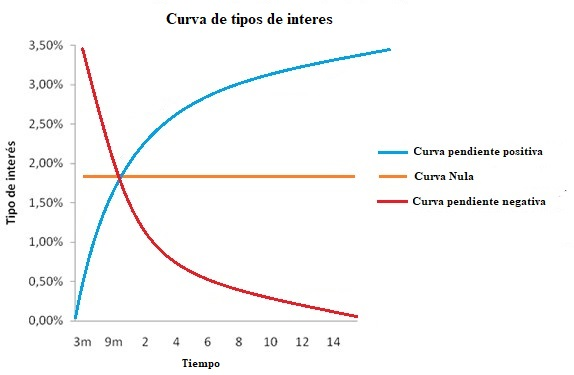
\includegraphics{images/tipo_curvas.jpg}}
\caption{Tipos de curva de rendimiento.}
\label{tipos_c}
\end{figure}

\hspace*{0.4 cm} Es de esperar que una pendiente negativa de la curva de rendimientos (Ver Figura \ref{tipos_c}) o curva invertida (tasas de largo plazo menores a las de corto plazo) indique expectativas de una recesi\'on futura y, por lo tanto, menores tasas de inter\'es futuras; esto se puede explicar ya que los rendimientos esperados contienen informaci\'on sobre los planes de consumo de los agentes. 

\hspace*{0.4 cm} Entre las teor\'ias que explican la pendiente de la curva de rendimientos, se encuentran:

\begin{itemize}
  \item \textbf{La teor\'ia de la preferencia por la liquidez}: consiste en que los inversionistas prefieren manejar t\'itulos a corto plazo, pues \'estos tienen una sensibilidad menor a los cambios en las tasas de inter\'es y ofrecen una mayor flexibilidad en las inversiones si se compara con los t\'itulos de largo plazo. Adem\'as, los prestatarios prefieren deuda a largo plazo, pues la de corto plazo los expone al riesgo de hacer una refinanciaci\'on de la deuda en condiciones adversas. Ambas situaciones, generan entonces, tasas de corto plazo relativamente bajas. En su conjunto, estos dos grupos de preferencias implican que en condiciones normales existe una Prima de Riesgo por Vencimiento (PRV) que aumenta en funci\'on de los a\~nos de vencimiento, haciendo que la curva de rendimientos posea una pendiente ascendente \cite{DO}.
  \item \textbf{La teor\'ia de la segmentaci\'on del mercado}: considera el mercado de renta fija como una serie de distintos mercados, los inversionistas y los emisores est\'an restringidos por el sector espec\'ifico de maduraci\'on. De acuerdo con esta teor\'ia, la curva de rendimientos refleja una serie de condiciones de oferta y demanda que crean una secuencia de precios de equilibrio de mercado (tasas de inter\'es) de los fondos \cite{DO}.
  \item \textbf{La teor\'ia del H\'abitat Preferido}: plantea que los inversionistas intentar\'an liquidar sus inversiones en el menor plazo posible mientras que los prestamistas querr\'an tomar un plazo m\'as largo; por lo tanto, dado que no se encuentran oferta y demanda de fondos para un mismo plazo, algunos inversionistas o prestatarios se ver\'an motivados a cambiar el plazo de la inversi\'on o el financiamiento pero, para lograrlo, deben ser compensados con un premio por el riesgo cuyo tamano reflejar\'a la extesi\'on de la aversi\'on al riesgo.
  \item \textbf{La Hip\'otesis de las Expectativas (HE)}: plantea que las tasas de inter\'es de largo plazo deben reflejar por completo la informaci\'on revelada por las futuras tasas de inter\'es de corto plazo esperadas \cite{YS}, o sea que los tipos de largo plazo no son m\'as que una suma ponderada de los tipos de corto plazo esperados \cite{FR}. As\'i, se puede afirmar entonces que la HE es una teor\'ia que plantea que las tasas de inter\'es exclusivamente representan las tasas previstas en el futuro.
\end{itemize}



\section{Deuda P\'ublica Nacional.}

\hspace*{0.4 cm} Uno de los principales objetivos que se persigue mediante el uso de la curva de rendimientos es el de estimar los precios de los t\'itulos de la deuda p\'ublica nacional que posee una instituci\'on financiera en su portafolio de inversiones en un per\'iodo determinado. 


% \hspace*{0.4 cm} Por una parte se tiene que deuda es la obligaci\'on que un sujeto tiene de reintegrar, satisfacer o pagar, especialmente dinero. P\'ublico, por otra parte, es un adjetivo que refiere a aquello perteneciente a toda la sociedad o que es com\'un del pueblo.

\hspace*{0.4 cm} La noci\'on de deuda p\'ublica hace menci\'on al conjunto de deudas que mantiene el Estado frente a otro pa\'is o particulares. Se trata de un mecanismo para obtener recursos financieros a trav\'es de la emisi\'on de t\'itulos de valores.

\hspace*{0.4 cm} El Estado, por lo tanto, contrae deuda p\'ublica para solucionar problemas de liquidez (cuando el dinero en caja no resulta suficiente para afrontar los pagos inmediatos) o para financiar proyectos a medio o largo plazo. La deuda p\'ublica puede ser contra\'ida por la administraci\'on municipal, provincial o nacional. Al emitir t\'itulos de valores y colocarlos en los mercados nacionales o extranjeros, el Estado promete un futuro pago con intereses seg\'un los plazos estipulados por el bono.

\hspace*{0.4 cm} La emisi\'on de deuda p\'ublica, al igual que la creaci\'on de dinero y los impuestos, son medios que tiene el Estado para financiar sus actividades. La deuda p\'ublica, de todos modos, tambi\'en puede utilizarse como un instrumento de la pol\'itica econ\'omica, de acuerdo a la estrategia escogida por las autoridades. Tendr\'iamos que hablar, por un lado, de tres tipos diferentes de deuda p\'ublica, aunque es cierto que hay diversas clasificaciones. Una clasificaci\'on de la deuda, es la siguiente,

\begin{itemize}
  \item \textbf{A corto plazo}: dentro de esta categor\'ia se encuentran las Letras del Tesoro y se identifica por el hecho de que tiene un plazo de vencimiento que no supera el a\~no.
  \item \textbf{A medio plazo}: los bonos del Estado son los m\'aximos exponentes de esta clase de deuda p\'ublica que se suele utilizar para hacer frente a lo que ser\'an los gastos ordinarios.
  \item \textbf{A largo plazo}: como su propio nombre indica, este tipo de deuda tiene una duraci\'on muy larga, que se fijar\'a convenientemente, y que puede incluso llegar a ser perpetua. 
\end{itemize}


\hspace*{0.4 cm} Otra posible clasificasi\'on de la deuda p\'ublica se presenta a continuaci\'on. La deuda p\'ublica real es aquella compuesta por los t\'itulos que pueden ser adquiridos por los particulares, los bancos privados y el sector exterior. La deuda p\'ublica ficticia, en cambio, es la emisi\'on destinada al Banco Central del pa\'is, que es un organismo de la misma administraci\'on p\'ublica.





% \hspace*{0.4 cm} Con el fin de calcular o estimar los precios de los t\'itulos \'o instrumentos de deuda p\'ublica nacional que existen en el mercado venezolano es importante conocer las caracter\'isticas de los mismos, entre ellos tenemos los siguientes,
% 
% \vspace{0.4cm}
% 
% \begin{itemize}
%   \item T\'itulos de inter\'es fijo (TIF): son instrumentos que se caracterizan por tener una renta fija, y se emiten en moneda nacional.
%   \item T\'itulos de inter\'es variable (VEBONO): se caracterizan por poseer una renta variable, e igual que los TIF se emiten en Bol\'ivares.
%   \item Bonos PDVSA : son instrumentos emitidos en d\'olares.
% \end{itemize}
% 
% \vspace{0.5cm}
% 
% \noindent cabe destacar que en el presente trabajo s\'olo  se considerar\'an aquellos instrumentos emitidos en Bol\'ivares.
% 
% \vspace{0.5cm}
% 
% \hspace*{0.4 cm}Asociado a cada t\'itulo hay un monto de dinero que se invierte, el cual es entregado al ente emisor por el t\'itulo en s\'i, existe tambi\'en una fecha de emisi\'on, y una fecha de vencimiento, d\'ia en el cual el ente emisor retorna el monto invertido inicialmente. Es importante destacar que estos t\'itulos pagan un inter\'es al portador cada tres meses, y esta representa la ganancia que tiene el inversionista.
% 
% \vspace{0.5cm}
% 
% \hspace*{0.4 cm} Con el fin de determinar en que t\'itulo es mejor invertir, es necesario conocer el rendimiento al vencimiento que posee dicho t\'itulo, este valor nos da un idea de cu\'al ser\'a el retorno que recibir\'a el portador del t\'itulo por la tenencia o compra del mismo. Para calcular este valor es necesario conocer la fecha de vencimiento del t\'itulo as\'i como su valor nominal y su precio.
% 
% 
%  \hspace*{0.4 cm} A partir de la siguiente f\'ormula podemos hallar dicho valor,
% 
% \vspace{0.5cm}
% 
% \begin{center}
% 
% $\displaystyle{P_{t,m} = \sum_{i=1}^{m-1}{\frac{c}{(1+R_{t,i})^i} + \frac{1+c}{(1+R_{t,m})^m}} }$
% 
% \end{center}
% 
% \vspace{0.5cm}
% 
% \noindent donde $P_{t,m}$ representa el precio del t\'itulo al tiempo t, y que tiene un vencimiento de m a\~nos, c representa el cup\'on asociado al t\'itulo, el \'indice $i = 1,...,m$ representa cuantos cupones todav\'ia le quedan al t\'itulo por pagar antes de su vencimiento. Por su parte $R_{t,m}$ representa el rendimiento al vencimiento del t\'itulo en el tiempo t y que tiene un vencimiento de m a\~nos.
% 
% \vspace{0.5cm}
% 
% \hspace*{0.4 cm}A partir de la f\'ormula anterior podemos afirmar que para calcular el rendimiento al vencimiento de un t\'itulo es necesario conocer su precio es una fecha espec\'ifica, pero esto no siempre es posible, esto se debe a las caracter\'isticas del mercado venezolano ya que son pocos los t\'itulos que cotizan y por ende no se conoce su precio. Dicho precio puede conocerse a diario mediante la informaci\'on suministrada en la pesta\~na ``0-22" del documento ``resumersec" del Banco Central de Venezuela, este ente publica cada d\'ia las operaciones realizadas con estos instrumentos, en este documento se puede obtener el precio de aquellos t\'itulos que coticen ese d\'ia, el problema radica en conocer los precios de aquellos t\'itulos que no est\'en en dicho documento.
% 
% 
% 
% \vspace{0.5cm}

\section{Metodolog\'ias de estimaci\'on de la curva de rendimientos.}

\hspace*{0.4 cm} La curva de rendimientos presenta emp\'iricamente una serie de dificultades, debido a que se construye a trav\'es de una serie de precios (tasas) de instrumentos financieros discontinuos en el tiempo que, por lo general, est\'an lejos de ser una curva suave. Para su estimaci\'on existen diversas metodolog\'ias, las param\'etricas y las no param\'etricas. Las metodolog\'ias param\'etricas se basan en modelos asociados a una familia funcional que obedece al comportamiento de alguna distribuci\'on de probabilidad, sobre la cual suponemos que las caracter\'isticas de la poblaci\'on de inter\'es pueden ser descritas. Es as\'i como, los modelos dise\~nados en este contexto, basados en regresi\'on, buscan describir el comportamiento de una variable de inter\'es con otras llamadas ex\'ogenas, a trav\'es de funciones de v\'inculo lineales o no lineales.


\section{Metodolog\'ias param\'etricas.}

\hspace*{0.4 cm} Estad\'isticamente, un modelo param\'etrico es una familia funcional que
obedece al comportamiento de alguna distribuci\'on de probabilidad, sobre la cual suponemos que las caracter\'isticas de la poblaci\'on de inter\'es
pueden ser descritas. Es as\'i como, los modelos dise\~nados en este contexto,
basados en regresi\'on, buscan describir el comportamiento de una
variable de inter\'es con otras llamadas ex\'ogenas, a trav\'es de funciones de
v\'inculo lineales o no lineales.

\subsection{La curva de Nelson-Siegel.\\} 

\hspace*{0.4 cm} Nelson y Siegel \cite{NS} introducen un modelo param\'etrico para el ajuste
de los rendimientos hasta la madurez de los bonos del tesoro de Estados
Unidos que se caracteriza por ser parsimonioso y flexible en modelar
cualquier forma t\'ipica asociada con las curvas de rendimientos. La estructura
param\'etrica asociada a este modelo permite analizar el comportamiento
a corto y a largo plazo de los rendimientos y ajustar -sin
esfuerzos adicionales-, curvas mon\'otonas, unimodales o del tipo S.


\hspace*{0.4 cm} Una clase de funciones que genera f\'acilmente las formas usuales de las
curvas de rendimientos es la asociada con la soluci\'on de ecuaciones en
diferencia. La teor\'ia de expectativas sobre la estructura de las tasas de
inter\'es promueve la investigaci\'on en este sentido, dado que si las tasas
spot son producidas por medio de una ecuaci\'on diferencial, entonces las
tasas forward -siendo pron\'osticos-, ser\'an la soluci\'on de las ecuaciones
diferenciales. La expresi\'on param\'etrica propuesta por Nelson y Siegel
\cite{NS} que describe las tasas forward es exhibida a continuaci\'on:


\begin{center}
$\displaystyle{f(m) = \beta_{0} + \beta_{1} e^{\frac{-m}{\tau}} +\beta_{2} \left(\frac{m}{\tau}\right)e^{\frac{-m}{\tau}}}$
\end{center}

\vspace*{0.2 cm}

\noindent donde $m$ denota la madurez del activo y $\beta_{0}$, $\beta_{1}$, $\beta_{2}$ y $\tau$ los par\'ametros a ser
estimados. La ecuaci\'on anterior es la soluci\'on de la ecuaci\'on diferencial homog\'enea de segundo orden $y'' + 2y' + 1 = 0$, la cual tiene por soluci\'on dos raices reales iguales. Puesto que las tasas spot pueden ser obtenidas a trav\'es de tasas
forward por medio de la expresi\'on:

\vspace*{0.2 cm}

\begin{center}
$\displaystyle{s(m) = \int_{0}^{m}f(x)dx}$
\end{center}

\vspace*{0.2 cm}


\noindent la ecuaci\'on que determina las tasas spot $s(m)$ de activos con madurez m es dada por:

\vspace*{0.2 cm}


\begin{center}
$\displaystyle{s(m) = \beta_{0}+ \beta_{1}\frac{\left(1-e^\frac{-m}{\tau}\right)}{m/\tau} + \beta_{2} \left(\frac{\left(1-e^\frac{-m}{\tau}\right)}{m/\tau} -  e^\frac{-m}{\tau}\right)}$
\end{center}

\vspace*{0.2 cm}

\noindent cuya ecuaci\'on es lineal si conocemos $\tau$ .

\hspace*{0.4 cm} El valor l\'imite del rendimiento es $\beta_{0}$ cuando el plazo al vencimiento $m$ es grande, mientras que, cuando el plazo al vencimiento $m$ es peque\~no el
rendimiento en el l\'imite es $\beta_{0}+\beta_{1}$. Igualmente, los coeficientes del
modelo de tasas forward pueden ser interpretados como medidas de
fortaleza al corto, mediano y largo plazo. La contribuci\'on al largo plazo
es determinada por $\beta_{0}$, $\beta_{1}$ lo hace al corto plazo ponderado por la
funci\'on mon\'otona creciente (decreciente) $e^{\frac{-m}{\tau}}$ cuando $\beta_{1}$ es negativo
(positivo) y $\beta_{2}$ lo hace al mediano plazo ponderado por la funci\'on
mon\'otona creciente (decreciente) $(\frac{-m}{\tau}) e^{\frac{-m}{\tau}}$ cuando $\beta_{2}$ es negativo
(positivo). Una de las principales utilidades de la curva ha sido para
prop\'ositos de control de la pol\'itica monetaria.

\hspace*{0.4 cm} Consecuentemente, $s(m)$ ser\'a la ecuaci\'on utilizada para captar la relaci\'on
subyacente entre los rendimientos y los plazos al vencimiento o madurez,
sin recurrir a modelos m\'as complejos que involucren un mayor n\'umero
de par\'ametros. Adicionalmente, dado que la curva de Nelson-Siegel
proporciona tasas spot compuestas continuas, estas deben transformarse
en cantidades discretas, a trav\'es de la funci\'on de descuento.


\begin{center}
$\displaystyle{s_{d}(m) = e^{\frac{s(m)}{100}} - 1}$
\end{center}

\subsection{La curva de Svensson.\\}

\hspace*{0.4 cm} En la curva de Nelson-Siegel se destaca que cada coeficiente del modelo
contribuye en el comportamiento de las tasas forward en el corto,
mediano y largo plazo; no obstante, Svensson \cite{Sv} propone una nueva
versi\'on de la curva de Nelson-Siegel donde un cuarto t\'ermino es incluido
para producir un efecto adicional y semejante al proporcionado por:
$\beta_{2}(\frac{m}{\tau_{1}})e^{\frac{-m}{\tau_{1}}}$.

\hspace*{0.4 cm} En este caso, la funci\'on para describir la din\'amica de las tasas forward es,

\vspace*{0.2 cm}

\begin{center}
$\displaystyle{f(m) = \beta_{0} + \beta_{1} e^{\frac{-m}{\tau_{1}}} +\beta_{2} \left(\frac{m}{\tau_{1}}\right)e^{\frac{-m}{\tau_{1}}} + \beta_{3}\left(\frac{m}{\tau_{2}}\right)e^{\frac{-m}{\tau_{2}}} }$
\end{center}

\vspace*{0.2 cm}

\hspace*{0.4 cm} La curva spot de Svensson puede ser derivada a partir de la curva
forward en forma semejante a la descrita para el modelo de Nelson-
Siegel, obteniendo la siguiente expresi\'on:

\vspace*{0.2 cm}

\begin{center}
$\displaystyle{s(m) = \beta_{0}+ \beta_{1}\frac{\left(1-e^\frac{-m}{\tau_{1}}\right)}{m/\tau_{1}} + \beta_{2} \left(\frac{\left(1-e^\frac{-m}{\tau_{1}}\right)}{m/\tau_{1}} -  e^\frac{-m}{\tau_{1}}\right) + \beta_{3} \left(\frac{\left(1-e^\frac{-m}{\tau_{2}}\right)}{m/\tau_{2}} -  e^\frac{-m}{\tau_{2}}\right)}$
\end{center}

\vspace*{0.2 cm}

\hspace*{0.4 cm} La funci\'on de descuento tiene que ser utilizada con el fin de obtener las
tasas estimadas para cada d\'ia de negociaci\'on o trading. Svensson \cite{Sv}
propone estimar los par\'ametros de la curva cero cup\'on (curva spot),
minimizando una medida de ajuste tal como la suma de cuadrados del
error sobre los precios spot; sin embargo, enfatiza en que los precios
pueden llegar a ser mal ajustados para los activos de madurez corta. En
lugar de llevar el an\'alisis por este camino, propone estimar los
rendimientos fundamentado, principalmente, en que las decisiones de la
pol\'itica econ\'omica se basan en el comportamiento de las tasas y que
obteniendo las tasas a trav\'es de la curva, los precios pueden ser
calculados una vez la funci\'on de descuento es evaluada. De esta manera,
los par\'ametros son escogidos minimizando la suma de cuadrados de la
diferencia entre los rendimientos observados y estimados por la curva.

\hspace*{0.4 cm} La estimaci\'on es realizada por medio de m\'axima verosimilitud, m\'inimos
cuadrados no lineales o el m\'etodo de momentos generalizados. En
muchos casos, como afirma Svensson \cite{Sv}, el modelo de Nelson-
Siegel proporciona ajustes satisfactorios, aunque en algunos casos
cuando la estructura de las tasas de inter\'es es m\'as compleja, el ajuste del
modelo de Nelson-Siegel es poco satisfactorio y el modelo de Svensson
logra desempe\~narse mejor.


\subsection{Polinomios de componentes principales.\\}


\hspace*{0.4 cm} Hunt y Terry \cite{HT} propone un ajuste de la curva de rendimientos
utilizando polinomios. Si frecuentemente la curva es especificada como,

\begin{equation}
y(\tau) = \beta_{0} + \beta_{1}\tau +\beta_{2}\tau^2 +\beta_{3}\tau^3
\label{cp}
\end{equation}


\hspace*{0.4 cm} La cual puede captar todas la formas que puede asumir la curva, su
principal problema recae en el ajuste para aquellas tasas con per\'iodos de
vencimiento bastante largos. Aunque los autores conocen sobre las
propiedades de parsimonia y de ajuste asociados con la curva de Nelson-
Siegel, critican los problemas que acarrea la estimaci\'on de sus
par\'ametros, proponiendo el ajuste de la curva de polinomios, bajo
algunas modificaciones.

\hspace*{0.4 cm} Una transformaci\'on sobre el t\'ermino de plazos ($\tau$) que remueve la
inestabilidad asociada con las tasas a largo plazo del polinomio de la ecuaci\'on (\ref{cp}) es
sugerida. El modelo recomendado, siguiendo la notaci\'on de Hunt y
Terry (1998) es:

\begin{equation}
y(\tau) = \beta_{0} + \sum_{i=1}^{p} \beta_{i} \frac{1}{(1+\tau)^i}
\label{cp1}
\end{equation} 

\noindent donde,

\begin{center}
$\displaystyle{y(0) = \sum_{i=0}^{p}\beta_{i} \hspace*{0.2 cm} y \hspace*{0.2 cm} y(\infty) = \beta_{0}   }$
\end{center} 

\vspace*{0.2 cm}

\hspace*{0.4 cm}Investigaciones relacionadas con curvas de rendimientos, han llegado a
la conclusi\'on que modelos con tres o cuatro par\'ametros son suficientes
para obtener un buen ajuste de los datos (Hunt \cite{H}). Por tal motivo,
Hunt y Terry \cite{HT} proponen restringir $p$ a tres o cuatro. Aunque este
n\'umero de par\'ametros no necesariamente determina si realmente la
bondad de ajuste pueda llegar a ser satisfactoria, los autores proponen
utilizar componentes principales sobre los primeros $p$ t\'erminos
polinomiales $1/(1 + \tau)$, con el fin de seleccionar $k<p$ variables, a ser
incluidas en la ecuaci\'on (\ref{cp1}). Utilizar las componentes principales
proporcionar\'a un menor error de ajuste en comparaci\'on con la ecuaci\'on (\ref{cp}),
debido a su capacidad para captar variabilidad. Una descripci\'on
detallada respecto al c\'alculo de las componentes principales en el
esquema polinomial es dada por Hunt y Terry \cite{HT}.

\subsection{Polinomios trigonom\'etricos.\\}



\hspace*{0.4 cm} Las funciones trigonom\'etricas pueden ser utilizadas para capturar de
forma satisfactoria las distintas configuraciones que pueden asumir las
curvas de rendimientos. En este caso, el modelo puede ser descrito como
$y(\tau) = \beta_{0} + \beta_{1}cos(\gamma_{1}\tau) + \beta_{2}sen(\gamma_{2}\tau)$; donde $\tau$ representa la duraci\'on o la
madurez del papel, en tanto que $\beta_{0}$, $\beta_{1}$, $\beta_{2}$, $\gamma_{1}$ y $\gamma_{2}$ son los par\'ametros
objeto de inter\'es. Cualquier metodolog\'ia de optimizaci\'on no lineal puede
ser utilizada para estimar los par\'ametros del modelo (Nocedal y Wright
\cite{NW}). Aunque podr\'ia asumirse un par\'ametro de fase en el modelo, este
no es considerado por motivos de parsimonia.

\section{Metodolog\'ias no param\'etricas}

\hspace*{0.4 cm} La regresi\'on no param\'etrica se ha convertido en los \'ultimos a\~nos en un
\'area de excesivo estudio, debido a sus ventajas relativas respecto a los
modelos de regresi\'on basado en funciones. Entre las caracter\'isticas m\'as
importantes de estos modelos tenemos, la flexibilidad en los supuestos y
el ajuste dirigido espec\'ificamente a trav\'es de los datos.


\hspace*{0.4 cm} Dentro de un marco estad\'istico supondremos que tenemos un conjunto
de n observaciones $(x_{i}, y_{i})$, $i= 1, 2,., n$, independientes, donde se intenta
establecer las relaciones existentes entre una respuesta y un conjunto de
variables explicativas de forma semejante a los modelos de regresi\'on
cl\'asica.


\hspace*{0.4 cm} El modelo que relaciona este conjunto de variables es dado por:

\begin{center}
$\displaystyle{y_{i} = m(x_{i}) + \epsilon_{i}}$
\end{center} 



\noindent donde la funci\'on $m(.)$ no espec\'ifica una relaci\'on param\'etrica, sino
permitir que los datos determinen la relaci\'on funcional apropiada. Bajo
estas condiciones la idea es que la media m(.) sea suave, suavidad que
puede controlarse acotando la segunda derivada, $|m''(x)| \leq M$, para todo
$x$ y $M$ una constante.

\subsection{Regresi\'on de n\'ucleo.\\}


\hspace*{0.4 cm} El m\'etodo m\'as simple de suavizamiento es el suavizador de n\'ucleo. Un
punto x se fija en el soporte de la funci\'on $m(.)$ y una ventana de
suavizamiento es definida alrededor de x. Frecuentemente, la ventana de
suavizamiento es simplemente un intervalo de la forma $(x - h, x + h)$,
donde h es un par\'ametro conocido como ancho de banda.

\hspace*{0.4 cm} La estimaci\'on de n\'ucleo es un promedio ponderado de las observaciones
dentro de la ventana de suavizamiento,

\begin{equation}
\hat{m}(x) = \frac{\sum_{i=1}^{n} K(\frac{x_{i}-x}{h}) y_{i}}{\sum_{i=1}^{n} K(\frac{x_{i}-x}{h})}
\label{kernel}
\end{equation}

\vspace*{0.2 cm}

\noindent donde $K(.)$ es la funci\'on de n\'ucleo de ponderaci\'on. La funci\'on de n\'ucleo es escogida
de tal forma que las observaciones m\'as pr\'oximas a x reciben mayor peso. Una
funci\'on frecuentemente utilizada es la bicuadr\'atica:

$$ K(x) = \left\{ % para la llave grandota
        \begin{tabular}{cc}
        	$(1-x^2)^2$ & si $-1 \leq x  \leq 1$ \\
        	$0$ & si $x \ge 1, \hspace*{0.2 cm} x<-1$ \\
        \end{tabular}
\right. $$

\vspace*{0.2 cm}

\hspace*{0.4 cm} Sin embargo, otro tipo de funciones de peso son utilizadas, tal como la
gaussiana, $K(x) = (2 \sqrt{\pi})^{-1} e^{\frac{-x^2}{2}}$ y la familia beta sim\'etrica $K(x) = \frac{(1-x^2)_{+}^{\gamma}}{Beta(0.5,\gamma+1)}, \hspace*{0.2 cm}\gamma = 0,1,...$

\hspace*{0.4 cm} Note que cuando escogemos $\gamma = 0, 1, 2$ y $3$ obtenemos las funciones de n\'ucleo uniforme (Box), de Epanechnikov, la bipeso y la tripeso, respectivamente.

\hspace*{0.4 cm} El suavizador de n\'ucleo puede ser representado como,

\vspace*{0.2 cm}


\begin{equation}
\hat{m}(x) = \sum_{i=1}^{n} l_{i}(x) y_{i} 
\label{kernel1}
\end{equation}

\vspace*{0.2 cm}

\noindent donde,

\vspace*{0.2 cm}

\begin{center}
$\displaystyle{l_{i} = \frac{K(\frac{x_{i}-x}{h})}{\sum_{j=1}^{n} K(\frac{x_{j}-x}{h})} }$
\end{center}

\vspace*{0.2 cm}


\hspace*{0.4 cm} La estimaci\'on de n\'ucleo en la ecuaci\'on (\ref{kernel}) es llamada la estimaci\'on de Nadaraya - Watson, en honor a sus creadores. Su simplicidad lo hace de f\'acil comprensi\'on e implementaci\'on; no obstante, se sabe que los ajustes en los extremos son sesgados. Una referencia ideal para un desarrollo m\'as completo sobre este tema puede encontrarse en Fan y Gijbels \cite{FG}.

\subsection{Polinomios locales.\\}



\hspace*{0.4 cm} Conocida tambi\'en como regresi\'on local, la idea es aproximar la funci\'on suave m(.) por medio de un polinomio de bajo orden en una vecindad entorno de un punto x. Por ejemplo, una aproximaci\'on lineal local es $m(x_{i}) \approx a_{0} + a_{1}(x_{i}-x)$ para $x - h \leq x_{i} \leq x+h$. Una aproximaci\'on local cuadr\'atica es:

\vspace*{0.2 cm}

\begin{center}
$\displaystyle{m(x_{i}) \approx  a_{0} + a_{1}(x_{i}-x) + \frac{a_{2}}{2}(x_{i}-x)^2}$
\end{center}

\vspace*{0.2 cm}

\hspace*{0.4 cm} La aproximaci\'on local puede ser ajustada a trav\'es de m\'inimos cuadrados ponderados localmente. Una funci\'on de n\'ucleo y un ancho de banda son definidos como en la regresi\'on de n\'ucleo. Los coeficientes $\hat{a}_{0}$ y $\hat{a}_{1}$, son escogidos de tal forma que se pueda minimizar la expresi\'on,

\vspace*{0.2 cm}

\begin{equation}
 \sum_{i=1}^{n} K(\frac{x_{i}-x}{h}) (y_{i}-a_{0}-a_{1}(x_{i}-x))^2 
 \label{kernel2}
\end{equation}

\vspace*{0.2 cm}


\hspace*{0.4 cm} Reescribiendo la ecuaci\'on (\ref{kernel2}) en t\'erminos matriciales obtenemos, $X^{T}W(\tilde{Y}-X \tilde{a})$. Donde X es la matriz dise\~no para cada regresi\'on lineal, $\tilde{a}$ el vector de
par\'ametros, W la matriz diagonal de pesos $K(\frac{x_{i}-x}{h})$ y $\tilde{Y}$ el vector de observaciones de orden n.


\hspace*{0.4 cm} El vector de par\'ametros estimado est\'a dado por $ \hat{\tilde{a}} = (X^{T}WX)X^{T}W \tilde{Y} $
y en forma semejante con la ecuaci\'on (\ref{kernel1}), tenemos que: $l(x)_{nx1} = e_{1}^{T} (X^{T}WX)X^{T} \tilde{Y}$ donde $e_{1}^{T}$
es un vector de ceros de tama\~no n, exceptuando la primera entrada cuyo valor es 1.

\hspace*{0.4 cm}Finalmente, la selecci\'on del h est\'a basado en procedimientos de bondad de ajuste que permite obtener el mejor modelo. Entre los m\'as utilizados sobresalen los m\'etodos de validaci\'on cruzada generalizada y plug-in, los cuales son descritos detalladamente en Fan y Gijbels \cite{FG}.

\subsection{Splines suavizados.\\}

\hspace*{0.4 cm} Las funciones polinomiales se caracterizan por tener todas las derivadas en cualquier punto de su soporte; no obstante, cuando ciertas funciones no poseen un alto grado de suavidad en determinados puntos, el ajuste debido a estas funciones de polinomios no siempre ser\'a satisfactoria en estos tramos.

\hspace*{0.4 cm} Para sobrellevar esta desventaja, el ajuste de polinomios de bajo orden localmente, con discontinuidades en ciertos puntos (nodos), resulta en el conocido m\'etodo de splines.

\subsection{Splines de polinomios.\\}


\hspace*{0.4 cm}Suponga que queremos aproximar la funci\'on $m(.)$ por una funci\'on spline. Frecuentemente, el spline c\'ubico es utilizado para esta aproximaci\'on, sin embargo, otro tipo de splines pueden ser definidos.


\hspace*{0.4 cm}Siguiendo la notaci\'on de Fan y Gijbels \cite{FG}, sea $t_{1}, t_{2}, t_{3},...,t_{J}$ el conjunto de nodos o knots en orden creciente, tal que en cada intervalo  ($-\infty$, $t_{1}$], $[t_{1}, t_{2}],..., [t_{J-1}, t_{J}]$, [$t_{J}, \infty$), funciones c\'ubicas continuas diferenciables son ajustadas. En este caso el espacio par\'ametrico es (J+4)-dimensional.

\hspace*{0.4 cm} Un conjunto de splines c\'ubicos son ampliamente utilizados en la obtenci\'on de la funci\'on de splines, estas son las bases de potencias. Las mismas se definen como sigue, $(x- t_{j})_{+}^{3}, j= 1,2,...,J,1,x,x^2,x^3$ donde $x_{+}$ es la parte positiva de x. As\'i por ejemplo, la funci\'on de suavizamiento puede ser expresada como,

\begin{equation}
m(x) = \sum_{j=1}^{J+4} \theta_{j}B_{j}(x) 
\label{bases}
\end{equation}

\noindent siendo $B_{j}(x), j = 1, 2,... , J+4$, la base polinomial descrita anteriormente.

\hspace*{0.4 cm} Los regresores definidos de esta forma pueden ocasionar problemas de estimaci\'on (multicolinealidad), motivo por el cual, los $B_{j}(x)$ son
redefinidos como,

\vspace*{0.2 cm}


\begin{center}
$\displaystyle{ B_{j}(x) = \frac{x-x_{j}}{x_{j+k-1}-x_{j}} B_{j,k-1}(x) + \frac{x_{j+k}-x}{x_{j+k}-x_{j}} B_{j+1,k-1}(x) }$
\end{center}

\vspace*{0.2 cm}


\noindent suponiendo que $B_{j,1}=1$ para $x_{j} \leq x \leq x_{j+1}$ y cero en caso contrario. El proceso de estimaci\'on de la ecuaci\'on (\ref{bases}) es realizado a trav\'es de m\'inimos cuadrados penalizados.

\hspace*{0.4 cm}Adicionalmente, una desventaja del m\'etodo, es su sensibilidad al n\'umero y ubicaci\'on de los nodos, motivo por el cual han sido propuestos diferentes procedimientos para su selecci\'on.

\subsection{Splines suavizados.\\}



\hspace*{0.4 cm}El proceso de suavizamiento a trav\'es de este m\'etodo est\'a basado en la minimizaci\'on de la func\'ion,

\begin{center}
$\displaystyle{ \sum_{i=1}^{n} (y_{i}-m(x_{i})^2 + \lambda \int m''(x)^2dx  }$
\end{center}

\vspace*{0.2 cm}

\noindent donde $\lambda$ es una constante especificada de suavizamiento. El mecanismo de optimizaci\'on intenta crear un balance entre el sesgo de estimaci\'on y la suavidad de la curva ajustada. El par\'ametro $\lambda$ puede asumirse variable (Abramovich y Steinberg \cite{AS}) y estimado a trav\'es de validaci\'on cruzada generalizada.

\subsection{Supersuavizador de Friedmann.\\}


\hspace*{0.4 cm} Las metodolog\'ias usuales de suavizamiento asumen que el par\'ametro suavizador es constante, factor que sumado a la forma de la curva subyacente puede hacer que surjan problemas, tal como el aumento en la varianza de la componente del error y/o a variaciones incontrolables de la segunda derivada de la funci\'on subyacente sobre el conjunto predictor. El suavizador propuesto por Friedman \cite{F} intenta corregir estos problemas, asumiendo que el ancho de banda es variable sobre el conjunto de predictores.


\hspace*{0.4 cm} Formalmente, se puede estimar un ancho de banda para cada $x$, al igual que el correspondiente valor \'optimo de suavizamiento, minimizando la expresi\'on $e^{2}(m,h) = E(Y - m(X|h(X)))^2$ con respecto a las funciones $m(x)$ y $h(x)$. La expresi\'on anterior puede reescribirse como,

\vspace*{0.2 cm}

\begin{equation}
e^{2}(m,h) = E(E(Y - m(X|h(X)))^2|X)
\label{friedman}
\end{equation}

\vspace*{0.2 cm}

\noindent de tal forma que podemos minimizar el error con respecto a $m$ y $h$ para cada valor de $x$.

\hspace*{0.4 cm} Como en el caso del ancho de banda constante, se comienza aplicando un suavizador lineal local muchas veces sobre diferentes valores discretos de $h$, $0 < h < n$. Friedman \cite{F} propone utilizar tres conjuntos de valores, $h=0,05n$, $h=0,2n$ y $h=0,5n$, los cuales llama suavizadores ``tweeter", ``midrange" \hspace*{0.01 cm} y ``woofer", respectivamente.

\hspace*{0.4 cm} Para estimar la ecuaci\'on (\ref{friedman}) se utiliza el residual de la validaci\'on cruzada de la ecuaci\'on (\ref{friedman1}) cuya descripci\'on completa puede encontrarse en Friedman \cite{F},

\vspace*{0.2 cm}

\begin{equation}
 r_{i}(h)= \frac{|y_{i}-m(x_{i}|h)|}{\left(1-\frac{1}{h}-\frac{(x_{i}-\bar{x}_{h})^2}{V_{h}}\right)}  
 \label{friedman1}
\end{equation}

\vspace*{0.2 cm}

\noindent siendo $\bar{x}_{h}$ y $V_{h}$, la media y varianza de los $x$, bajo un $h$ preeestablecido. Igualmente, Friedman \cite{F} aconseja suavizar $|r_{i}(h)|$ contra $x_{i}$, utilizando los $\hat{e}(m, h|x_{i})$, en procura de seleccionar la mejor amplitud de intervalo o bandwith, $\hat{e}(m, h_{vc}(x_{i})|x_{i})=min_{h} \hat{e}(m, h|x_{i})$, donde $h_{vc} (x_{i})$ es el mejor ancho de banda bajo la validaci\'on cruzada respecto a cada $x_{i}$ , mientras que $h$ toma los valores de los suavizadores antes definidos.

\hspace*{0.4 cm} De esta manera, el mejor valor suavizado dado $x_{i}$, siguiendo la notaci\'on de Friedman \cite{F}, $s^{*}(x_{i})$, estar\'a asociado con el ancho de banda: ``tweeter", ``midrange" \hspace*{0.01 cm} o ``woofer" que minimice el error bajo la validaci\'on cruzada. Es posible a trav\'es de esta metodolog\'ia obtener para cada vecindad en torno a $x_{i}$ diferentes anchos de banda y suavizados que proporcionan resultados \'optimos, por tal raz\'on, Friedman \cite{F} propone seleccionar la mejor amplitud de intervalo, suavizando los $h_{vc} (x_{i})$ contra $x_{i}$ utilizando el suavizador ``midrange", mientras que la curva estimada es obtenida interpolando entre los dos suavizadores con los anchos de banda estimados m\'as parecidos.


\hspace*{0.4 cm} Una suposici\'on general establece que la curva subyacente que describe el comportamiento de los datos es suave, as\'i que ser\'ia posible modificar el ancho de banda en procura de un mayor suavizamiento, sacrificando exactitud num\'erica. Con este fin, Friedman \cite{F} propone un m\'etodo de c\'alculo del ancho de banda,

\vspace*{0.2 cm}

\begin{center}
$\displaystyle{h(x_{i}) = h_{vc}(x_{i}) + (h_{w} - h_{vc}(x_{i}))R_{i}^{10-\alpha}}$
\end{center}

\vspace*{0.2 cm}

\noindent con, 

\vspace*{0.2 cm}

\begin{center}
$\displaystyle{R_{i} = \left[\frac{\hat{e}(h_{vc}(x_{i})|x_{i})}{\hat{e}(h_{w}(x_{i})|x_{i})} \right] }$
\end{center}

\vspace*{0.2 cm}

\noindent donde $0 < \alpha < 10$, $h_{w}$ es la amplitud calculada utilizando 
el suavizador ``woofer"\hspace*{0.01 cm} y $h_{vc}(.)$ la amplitud obtenida bajo la validaci\'on cruzada para cada observaci\'on. Sin importar el $\alpha$, cuando la contribuci\'on relativa de cada una de estas amplitudes no difiere significativamente, la amplitud de intervalo o bandwidth seleccionada es la determinada por el suavizador ``woofer"\hspace*{0.01 cm}; no obstante, si la eficiencia relativa est\'a asociada con la amplitud bajo la validaci\'on cruzada, entonces, la ecuaci\'on en proporcionar\'a esta amplitud. En otros casos, dependiendo del desempe\~no relativo y el par\'ametro $\alpha$ definido por el usuario, la ecuaci\'on proporcionar\'a una amplitud, resultado de la combinaci\'on lineal entre el suavizador ``woofer" \hspace*{0.01 cm} y el obtenido bajo validaci\'on cruzada.

\hspace*{0.4 cm} Una vez el ancho de banda de suavizaci\'on variable ha sido obtenido, los siguientes pasos son realizados sobre el conjunto de observaciones,

\begin{itemize}
  \item[1)] Suavice los datos con los anchos de banda ``tweeter"\hspace*{0.01 cm}, ``midrange"\hspace*{0.01 cm} y ``woofer"\hspace*{0.01 cm}.
  \item[2)] Suavice los residuales absolutos (12) obtenidos bajo cada ancho de banda en el paso anterior, utilizando una amplitud de intervalo ``midrange"\hspace*{0.01 cm}.
  \item[3)] Seleccione el mejor ancho de banda para cada observaci\'on, minimizando el error sobre la salida del paso (2).
  \item[4)] Suavice los mejores anchos de banda estimados en el paso (3) utilizando amplitud de intervalo ``midrange"\hspace*{0.01 cm}.
  \item[5)] Utilice los anchos de banda suavizados para interpolar entre los valores suavizados obtenidos en el paso 1.
\end{itemize}


\hspace*{0.4 cm} Las principales deficiencias atribuidas a esta t\'ecnica est\'an asociadas con la p\'erdida de independencia entre los residuales $\epsilon_{i}$ relativo al orden de los predictores $x_{i}$, subestimando (sobre-estimando) cuando la correlaci\'on es positiva-alta (negativa-alta).

\subsection{Redes neuronales artificiales.\\}


\hspace*{0.4 cm} Los recientes desarrollos investigativos han mostrado la capacidad de las redes neuronales para la detecci\'on de patrones, clasificaci\'on y predicci\'on a trav\'es del aprendizaje por medio de la experiencia. Su importancia actual, sin lugar a dudas, es consecuencia del desarrollo computacional, punto de partida para su divulgaci\'on, desenvolvimiento te\'orico y pr\'actico en diversos campos del conocimiento.

\hspace*{0.4 cm} Una de las mayores \'areas de aplicaci\'on de las redes neuronales es la predicci\'on (Sharda \cite{SH}). Dentro de este contexto, las redes resultan ser una herramienta atractiva para los investigadores, comparada con las metodolog\'ias tradicionales basada en modelos de funciones.

\hspace*{0.4 cm} Las redes neuronales artificiales intentan emular el comportamiento biol\'ogico del cerebro humano. Como sabemos, el cerebro humano es un conjunto complejo de interconexiones de elementos simples llamados nodos o neuronas. Cada nodo recibe una se\~nal de entrada proveniente de otros nodos o a trav\'es de est\'imulos externos; localmente el nodo procesa la informaci\'on recibida por medio de una funci\'on de transferencia o activaci\'on y produce una se\~nal de salida transformada, que ir\'a hacia otros nodos o como una respuesta, consecuencia de un est\'imulo. Aunque cada nodo individualmente no proporciona informaci\'on realmente valiosa, en conjunto, pueden realizar un sorprendente n\'umero de tareas de forma eficiente. Esta caracter\'istica hace de las redes neuronales un mecanismo poderoso computacionalmente para aprender a partir de ejemplos y despu\'es generalizar para casos nunca antes considerados.


\hspace*{0.4 cm} Aunque diferentes arquitecturas de redes neuronales han sido propuestas (Haykin \cite{Ha}), la m\'as utilizada es la red multilayer Perceptron (MLP). Una red MLP est\'a compuesta de varias capas y nodos o neuronas. Los nodos de la primera capa son los encargados de recibir la informaci\'on del exterior, mientras que la \'ultima capa es encargada de proporcionar la respuesta asociada a esta informaci\'on. Entre estas dos capas puede haber innumerables capas y nodos. Adicionalmente, los nodos de capas adyacentes est\'an completamente conectados.

\hspace*{0.4 cm} Para un problema de pron\'ostico con redes neuronales, las entradas a la red son asociadas con variables independientes o explicativas. En este caso la relaci\'on funcional estimada establecida por la red neuronal ser\'a de la forma $y_{t}=f(x_{1}, x_{2},..., x_{p})$; donde $x_{1}, x_{2},..., x_{p}$ son p variables ex\'ogenas y y una variable end\'ogena. En este sentido la red es equivalente a un modelo de regresi\'on no lineal. Igualmente, en el contexto del pron\'ostico de series temporales, las entradas de la red son series rezagadas de la original y la salida representa su valor futuro. En este caso la red har\'ia un mapeo de la siguiente forma $y_{t}= f (y{t-1}, y{t-2}, ..., y{t-p})$, donde $y_{t}$ es la observaci\'on en el tiempo t. Bajo estas caracter\'isticas la red asemeja un modelo autorregresivo en el pron\'ostico de series temporales. Una discusi\'on respecto a la relaci\'on existente entre las redes neuronales y la metodolog\'ia de Box-Jenkins es dada por Suykens, Vandewalle y Moor \cite{SVM}.

\hspace*{0.4 cm} Antes de que la red sea utilizada para realizar alguna tarea espec\'ifica, debe ser entrenada. B\'asicamente, entrenar es el proceso de determinar los pesos (eje central de la red neuronal). El conocimiento aprendido por la red es almacenado en cada una de los arcos que representan las conexiones entre los nodos. Es a trav\'es de estas conexiones que las redes pueden realizar complejos mapeos no lineales desde los nodos de entrada hasta los nodos de salida. El entrenamiento de la MLP es supervisado, caso en el cual la respuesta deseada o valor objetivo para cada patr\'on de entrada o ejemplo est\'a siempre disponible.

\hspace*{0.4 cm} Los datos de entrenamiento son ingresados a la red en forma de vectores de variables o como patrones de entrada. Cada elemento en el vector de entrada es asociado con un nodo de la capa de entrada; de esta forma, el n\'umero de entradas a la red es igual a la dimensi\'on del vector de entrada. Para el pron\'ostico de series temporales el n\'umero de variables de entrada es dif\'icil de establecer, no obstante, una ventana de rezagos fija es constituida a lo largo de la serie. El total de datos disponible es usualmente dividido en un conjunto de entrenamiento y otro de prueba. El primero es utilizado para estimar los pesos de la red, mientras que el segundo es empleado para evaluar la capacidad de generalizaci\'on de la red.


\hspace*{0.4 cm} Para el proceso de entrenamiento, patrones de entrada son ingresados a la red. Los valores de activaci\'on de los nodos de entrada son multiplicados por su peso respectivo y acumulados en cada nodo sobre la primera capa. El total es evaluado en una funci\'on de activaci\'on y asumido como la salida del respectivo nodo. A esta salida algunos investigadores la identifican como la activaci\'on del nodo y es la entrada de otros nodos en capas siguientes de la red hasta que los valores de activaci\'on de la salida sean encontrados. El algoritmo de entrenamiento es utilizado para encontrar los pesos que minimicen una medida global de error tal como la suma de cuadrados del error (SSE, por sus siglas en ingles).


\hspace*{0.4 cm} En el pron\'ostico con series temporales, un patr\'on de entrenamiento consiste de un conjunto de valores fijos de variables en rezago de la serie. Suponga que tenemos N observaciones $y_{1}, y_{2}, ..., y_{N}$ para el proceso de entrenamiento y se requiere pronosticar un paso al frente, entonces con una red neuronal de n nodos de entrada, tenemos $N-n$ patrones de entrenamiento. El primer patr\'on de entrenamiento estar\'a conformado por $y_{1}, y_{2}, ..., y_{n}$ como las entradas y $y_{n+1}$ como el valor objetivo. El segundo patr\'on de entrenamiento ser\'a $y_{2}$, $y_{3}$, ..., $y_{n+1}$ y el valor de salida deseado $y_{n+2}$. Finalmente, el \'ultimo patr\'on de entrada ser\'a $y_{N-n}, y_{N-n+1}, ..., y_{N-1}$ y $y_{N}$ el valor objetivo. Frecuentemente, una funci\'on objetivo basada en la SSE es minimizada durante el proceso de entrenamiento,

\vspace*{0.2 cm}

\begin{center}
$\displaystyle{E = \frac{1}{2} \sum_{i=n+1}^{N}(y{i}-a{i})^2 }$
\end{center}

\vspace*{0.2 cm}


\noindent  donde $a_{i}$ es la salida actual de la red.

\hspace*{0.4 cm}Una descripci\'on m\'as detallada sobre las diferentes arquitecturas de red existentes, el n\'umero \'optimo de capas ocultas y neuronas, las funciones de activaci\'on m\'as utilizadas, los algoritmos de entrenamiento, la normalizaci\'on de los datos, como tambi\'en de otros temas relacionados con sus ventajas y deficiencias (Haykin \cite{Ha}, Kaastra y Boyd \cite{KB}, Zhang, Patuwo y Hu \cite{ZPH}, Isasi y Galv\'an \cite{IG}), entre otros.



% \hspace*{0.4 cm} Por su parte, las metodolog\'ias no param\'etricas se han convertido en los \'ultimos a\~nos en un
% \'area de gran estudio debido a sus ventajas relativas respecto a los modelos de regresi\'on basado en funciones. Entre las caracter\'isticas m\'as importantes de estos modelos tenemos, la flexibilidad en los supuestos y el ajuste dirigido espec\'ificamente a trav\'es de los datos. Entre estas metodolog\'ias se destacan la de regresi\'on Kernel, polinomios locales, splines de polinomios (Fan y Gibels, $1996$ [6]), splines c\'ubicos suavizados (B.W. Silverman, $1985$ [7]), super suavizador de Friedmann (Friedmann, $1984$ [8]) y redes neuronales artificiales (Sharda, $1994$ [9]).
% 
% \vspace{0.5cm}
% 
% \hspace*{0.4 cm} En el siguiente trabajo se propone el uso de la metodolog\'ia de splines c\'ubicos suavizados, la cual posee la ventaja de contar un factor de penalizaci\'on el cu\'al es muy \'util al momento de tener un balance entre la suavidad de la curva y su bondad de ajuste. A grandes rasgos estas metodolog\'ias se basan en estimar la curva de rendimientos de dichos t\'itulos, curva que relaciona el rendimiento al vencimiento con la maduraci\'on o fecha de vencimiento, con el fin de estimar los precios de los t\'itulos a un d\'ia en espec\'ifico. De esta manera a partir de una determinada fecha es posible mediante estas metodolog\'ias estimar el rendimiento al vencimiento de un t\'itulo y por ende saber su precio estimado.

\newpage

\section{Objetivos.}

\subsection{Objetivos  generales del trabajo.}

\begin{itemize}
  \item Estimar la curva de rendimientos mediante el uso de los splines c\'ubicos suavizados.
\end{itemize}

\subsection{Objetivos espec\'ificos del trabajo.}

\begin{itemize}
  \item Generar un hist\'orico para los t\'itulos de tasa de inter\'es fija (TIF), pertenecientes a la deuda p\'ublica nacional (DPN).
  \item Estimar la curva de rendimientos para los TIF.
  \item Generar un hist\'orico para los t\'itulos de tasa de inter\'es variable (VEBONO), pertenecientes a la deuda p\'ublica nacional (DPN).
  \item Estimar la curva de rendimientos para los VEBONO.
  \item Estimar los precios de los TIF pertenecientes a un portafolio en un momento espec\'ifico.
  \item Estimar los precios de los VEBONO pertenecientes a un portafolio en un momento espec\'ifico.

\end{itemize}





\chapter{Marco te\'orico.}

\section{Teor\'ia de interpolaci\'on.}

\hspace{0.4cm} En el subcampo matem\'atico del an\'alisis num\'erico, se denomina interpolaci\'on a la obtenci\'on de nuevos puntos partiendo del conocimiento de un conjunto discreto de puntos.


\hspace{0.4cm} En ciertos casos el usuario conoce el valor de una funci\'on $f(x)$ en una serie de puntos $x_{1}, x_{2},..., x_{N}$, pero no se conoce una 
expresi\'on anal\'itica de $f(x)$ que permita calcular el valor de la funci\'on para un punto arbitrario. Un ejemplo claro son las mediciones de laboratorio, donde se mide cada minuto un valor, pero se requiere el valor en otro punto que no ha sido medido. Otro ejemplo son mediciones de temperatura en la superficie
de la Tierra, que se realizan en equipos o estaciones meteorol\'ogicas y se necesita calcular la temperatura en un punto cercano, pero distinto al punto de medida.

\hspace{0.4cm} La idea de la interpolaci\'on es poder estimar $f(x)$ para un valor de x arbitrario, a partir de la construcci\'on de una curva o superficie que une los puntos donde se han realizado las mediciones y cuyo valor si se conoce. Se asume que el punto arbitrario x se encuentra dentro de los l\'imites de los puntos de medici\'on, en caso contrario se llamar\'ia extrapolaci\'on. 

\hspace{0.4cm} Un proceso de interpolaci\'on se realiza en dos etapas:

\begin{itemize}
  \item Hacer un ajuste de los datos disponibles con una funci\'on interpolante.
  \item Evaluar la funci\'on interpolante en el punto de inter\'es x.
\end{itemize}


\hspace{0.4cm} Este proceso en dos etapas no es necesariamente el m\'as 
eficiente. La mayor\'ia de algoritmos comienzan con un punto cercano $f(x_{i})$, y poco a poco van aplicando correcciones m\'as pequenas a medida que la 
informaci\'on de valores $f(xi)$ m\'as distantes son incorporadas. El procedimiento toma aproximadamente $O(N^{2})$ operaciones. Si la funci\'on tiene un comportamiento suave, la \'ultima correci\'on ser\'a la m\'as pequena y puede ser utilizada para estimar un l\'imite a rango de error.


\hspace{0.4cm} Dentro de las intepolaciones m\'as usadas podemos destacar,

\begin{itemize}
  \item Interpolaci\'on lineal
  \item Interpolaci\'on de Hermite
  \item Interpolaci\'on polin\'omica 
  \item Interpolaci\'on de Splines 

\end{itemize}

Interpolaci\'on lineal

\hspace{0.4cm} La interpolaci\'on lineal es un procedimiento muy utilizado para estimar los valores que toma una funci\'on en un intervalo del cual conocemos sus valores en los extremos $(x_{1}, f(x_{1}))$ y $(x_{2},f(x_{2}))$. Para estimar este valor utilizamos la aproximaci\'on a la funci\'on f(x) por medio de una recta $r(x)$ (de ah\'i el nombre de interpolaci\'on lineal, ya que tambi\'en existe la interpolaci\'on cuadr\'atica). 


\hspace{0.4cm} La expresi\'on de la interpolaci\'on lineal se obtiene del polinomio interpolador de Newton de grado uno. Aunque s\'olo existe un \'unico polinomio que interpola una serie de puntos, existen diferentes formas de calcularlo. Este m\'etodo es \'util para situaciones que requieran un n\'umero bajo de puntos para interpolar, ya que a medida que crece el n\'umero de puntos, tambi\'en lo hace el grado del polinomio.

\hspace{0.4cm} Existen ciertas ventajas en el uso de este polinomio respecto al polinomio interpolador de Lagrange. Por ejemplo, si fuese necesario a\~nadir alg\'un nuevo punto o nodo a la funci\'on, tan s\'olo habr\'ia que calcular este \'ultimo punto, dada la relaci\'on de recurrencia existente y demostrada anteriormente.

\hspace{0.4cm}El primer paso para hallar la f\'ormula de la interpolaci\'on es definir la pendiente de orden n de manera recursiva, as\'i,

\begin{itemize}
  \item $f_{0}(x_{i})$ es el t\'ermino i-\'esimo de la secuencia. 
  \item $\displaystyle{f_{1}(x_{0},x_{1}) = \frac{f_{0}(x_{1})-f_{0}(x_{0})}{x_{1}-x_{0}}}$
  \item $\displaystyle{f_{2}(x_{0},x_{1},x_{2}) = \frac{f_{1}(x_{1},x_{2})-f_{1}(x_{0},x_{1})}{x_{2}-x_{0}}}$
\end{itemize}

\hspace{0.4cm} En general,

\begin{center}
$\displaystyle{f_{i}(x_{0},x_{1},...,x_{i-1},x_{i}) = \frac{f_{i-1}(x_{1},...,x_{i-1},x_{i})-f_{i-1}(x_{0},x_{1},...,x_{i-1} )}{x_{i}-x_{0}}}$
\end{center}


\noindent donde  $\displaystyle{x_{i}-x_{j}}$ representa la distancia entre dos elementos.

\hspace{0.4cm} Puede apreciarse c\'omo en la definici\'on general se usa la pendiente del paso anterior, $f_{i-1}(x_{1},...,x_{i-1},x_{i})$, a la cual se le resta la pendiente previa de mismo orden, es decir, el sub\'indice de los t\'erminos se decrementa en 1, como si se desplazara, para obtener $f_{i-1}(x_{0},x_{1},...,x_{i-1})$.

\hspace{0.4cm} N\'otese tambi\'en que aunque el t\'ermino inicial siempre es $x_{0}$ este puede ser en realidad cualquier otro, por ejemplo, se puede definir $f_{1}(x_{i-1},x_{i})$ de manera an\'aloga al caso mostrado arriba.

\hspace{0.4cm} Una vez conocemos la pendiente, ya es posible definir el polinomio de grado n de manera tambi\'en recursiva, as\'i,

\begin{itemize}
  \item $p_{0}(x) = f_{0} (x_{0}) =x_{0}$.  Se define as\'i ya que este valor es el \'unico que se ajusta a la secuencia original para el primer t\'ermino. 
  \item $\displaystyle{p_{1}(x) = p_{0}(x) +  f_{1} (x_{0},x_{1}) (x-x_{0})}$.
  \item $\displaystyle{p_{2}(x) = p_{1}(x) +  f_{2} (x_{0},x_{1},x_{2}) (x-x_{0})(x-x_{1})}$.
\end{itemize}

\hspace{0.4cm} En general,

\begin{center}
$\displaystyle{p_{i}(x) = p_{i-1}(x) +  f_{i} (x_{0},x_{1},...,x_{i-1},x_{i}) \prod_{j=0}^{i-1}(x-x_{j})}$
\end{center}


Interpolaci\'on de Lagrange

\hspace{0.4cm} Empezamos con un conjunto de $n+1$ puntos en el plano (que tengan diferentes coordenadas x), $(x_{0}, y_{0}), (x_{1}, y_{1}), (x_{2}, y_{2}),...,(x_{n}, y_{n})$. As\'i, queremos encontrar una funci\'on polin\'omica que pase por esos $n+1$ puntos y que tengan el menor grado posible. Un polinomio que pase por varios puntos determinados se llama un polinomio de interpolaci\'on.

\hspace{0.4cm} Una posible soluci\'on viene dada por el  polinomio de interpolaci\'on de Lagrange. Lagrange public\'o su f\'ormula en 1795 pero ya hab\'ia sido publicada en 1779 por Waring y redescubierta por Euler en 1783.

\hspace{0.4cm} Dado un conjunto de $k + 1$ puntos $(x_{0}.x_{1}),...,(x_{k}.x_{k+1})$, donde todos los $x_{j}$ se asumen distintos, el polinomio interpolador en la forma de Lagrange es la combinaci\'on lineal,

\begin{center}
$\displaystyle{L(x) = \sum_{j=0}^{k} y_{j} l_{j}(x)}$
\end{center}


\noindent donde $ l_{j}(x)$ son las bases polin\'omicas de Lagrange ,

\begin{center}
$\displaystyle{l_{j}(x) = \prod_{i=0,i \neq j}^{k} \frac{x-x_{i}}{x_{j}-x_{i}}  }$
\end{center}

\hspace{0.4cm} La funci\'on que estamos buscando es una funci\'on polin\'omica $L(x)$ de grado $k$ con el problema de interpolaci\'on puede tener tan solo una soluci\'on, pues la diferencia entre dos tales soluciones, ser\'ia otro polinomio de grado $k$ a lo sumo, con $k+1$ ceros. Por lo tanto, $L(x)$ es el \'unico polinomio interpolador.


\hspace{0.4cm} Si se aumenta el n\'umero de puntos a interpolar (o nodos) con la intenci\'on de mejorar la aproximaci\'on a una funci\'on, tambi\'en lo hace el grado del polinomio interpolador as\'i obtenido, por norma general. De este modo, aumenta la dificultad en el c\'alculo, haci\'endolo poco operativo manualmente a partir del grado 4, dado que no existen m\'etodos directos de resoluci\'on de ecuaciones de grado 4, salvo que se puedan tratar como ecuaciones bicuadradas, situaci\'on extremadamente rara.

\hspace{0.4cm} La tecnolog\'ia actual permite manejar polinomios de grados superiores sin grandes problemas, a costa de un elevado consumo de tiempo de computaci\'on. Pero, a medida que crece el grado, mayores son las oscilaciones entre puntos consecutivos o nodos. Se podr\'ia decir que a partir del grado 6 las oscilaciones son tal que el m\'etodo deja de ser v\'alido, aunque no para todos los casos.

\hspace{0.4cm} Sin embargo, pocos estudios requieren la interpolaci\'on de tan s\'olo 6 puntos. Se suelen contar por decenas e incluso centenas. En estos casos, el grado de este polimonio ser\'ia tan alto que resultar\'ia inoperable. Por lo tanto, en estos casos, se recurre a otra t\'ecnica de interpolaci\'on, como por ejemplo a la Interpolaci\'on polin\'omica de Hermite o a los splines c\'ubicos. Otra gran desventaja, respecto a otros m\'etodos de interpolaci\'on, es la necesidad de recalcular todo el polinomio si se var\'ia el n\'umero de nodos.

\hspace{0.4cm} Aunque el polinomio interpolador de Lagrange se emplea mayormente para interpolar funciones e implementar esto f\'acilmente en una computadora, tambi\'en tiene otras aplicaciones en el campo del \'algebra exacta, lo que ha hecho m\'as c\'elebre a este polinomio, por ejemplo en el campo de los proyectores ortogonales.


Interpolaci\'on de Hermite

\hspace{0.4cm} El objetivo de esta interpolaci\'on Hermite es minimizar el error producido en la interpolaci\'on de Lagrange de la funci\'on $f(x)$ sobre el intervalo $[a, b]$ sin aumentar el grado del polinomio interpolador.


\hspace{0.4cm} Dados un entero no negativo N y  N + 1 puntos $(x_{0},..., x_{N})$ de la recta distintos dos a dos y los valores $f^{(j)} (x_{i})$, donde $0<i<N$ y $0<j<k_{i-1}$ de una funci\'on f y de sus derivadas, encontrar un polinomio de grado $m = (k_{0} +k_{1} +...+k_{n-1},)$ tal que,

\begin{center}
$\displaystyle{P^{(j)} (x_{i}) = f^{(j)} (x_{i}), para \hspace{0.2cm} 0<i<N \hspace{0.2cm}y \hspace{0.2cm} 0<j<k_{i-1}}$
\end{center}

\hspace{0.4cm} El problema de interpolaci\'on de Hermite tiene soluci\'on \'unica, que se llama polinomio interpolador de Hermite. En lugar de interpolar sobre un soporte de puntos (de Tchebycheff) donde en general se desconoce el valor de la funci\'on, de hace de otra manera, imponiendo unas condiciones al polinomio,

\begin{itemize}
  \item  Igualar el valor de la funci\'on en en los puntos del soporte, $P (x_{i}) = f^{(j)}$
  \item Igualar el valor de algunas derivadas de la funci\'on tambi\'en en los puntos del soporte, $P^{(j)} (x_{i}) = f^{(j)} (x_{i})$
\end{itemize}

\hspace{0.4cm} Por lo que podemos dejar el polinomio de Hermite de grado (n-1) expresado de la siguiente manera,

\begin{center}
$\displaystyle{L(x) = \sum_{j=0}^{k} y_{j} l_{j} (x) }$
\end{center}

\noindent donde $l_{j}(x)$ son los polinomios de la base de Lagrange.


Interpolaci\'on Polin\'omica

\hspace{0.4cm}Asumamos que se tiene una tabla con n puntos, $(x_{1},y_{1})...,(x_{n},y_{n})$, donde los valores $x_{i}$, para $i=1,...,n$ est\'an ordenados de forma creciente y todos ellos son distintos. Supongamos que dichos puntos se representan en un plano cartesiano y se quiere determinar una curva suave que interpole dichos valores. As\'i, se desea determinar una curva que est\'e definida para todos los $x$ y tome los valores correspondientes de $y$, esto es, que interpole todos los datos de la tabla. Cabe destacar que los puntos considerados se les conoce como nodos.


\vspace{0.5cm}

\hspace{0.4cm} La primera idea natural es usar una funci\'on polinomial que represente esta curva, la cual se puede representar como sigue,

\vspace{0.5cm}
\begin{center}

$\displaystyle{P_{n} = \sum_{i=0}^{n-1} a_{i}x^{i}}$

\end{center}

\noindent tal curva se le conoce como funci\'on polinomial interpoladora de grado n. N\'otese que en cada nodo se satisface que $P_{n}(x_{k})=y_{k}$, donde $k=1,...,n$.

\vspace{0.5cm}

\hspace{0.4cm} As\'i, se tiene que si la tabla es representada mediante una funci\'on subyacente $f(x)$ tal que $f(x_{k})=y_{k}$, para todo k, entonces esta funci\'on puede ser aproximada mediante $P_{n}$, en los puntos intermedios.


\vspace{0.5cm}

\hspace{0.4cm} No ser\'ia descabellado pensar que a medida que los nodos se incrementan, la aproximaci\'on ser\'ia cada vez mejor, lamentablemente esto no siempre es cierto, debido a que en el caso de tener una data con mucho ruido la interpolaci\'on no tendr\'ia mucho sentido ya que la varianza de los valores interpolados ser\'ia muy grande. En este caso, los polinomios interpoladores resultantes ser\'ian una mala representaci\'on de la funci\'on subyacente.

\vspace{0.5cm}

\hspace{0.4cm} Para evitar este fen\'omeno, puede ser de utilidad relajar la condici\'on de que $f(x)$ deber\'ia ser una funci\'on que interpole todos los valores dados y en su lugar usar un trozo de un polinomio local de interpolaci\'on. La funci\'on mediante la cual se logra esta interpolaci\'on se le conoce como spline.


\section{Splines.}

\vspace{1 cm}

\hspace{0.4cm} Una funci\'on spline $S(x)$ es una funci\'on que consta de trozos de polinomios unidos por ciertas condiciones de suavizado. Un ejemplo simple, es una funci\'on poligonal (spline de primer grado), la cual se forma por polinomios lineales unidos, los cuales se definen entre cada par de nodos. Entre los nodos $x_{j}$ y $x_{j+1}$ se define un spline de primer grado como sigue, \\

\begin{center}

$\displaystyle{S(x) = a_{j}x + b_{j} = S_{j}(x)}$

\end{center}

\vspace{0.5cm}

\noindent este spline es lineal. Usualmente $S(x)$ se define como $S_{1}(x)$ para $x<x_{1}$ y como $S_{n-1}(x)$ para $x>x_{n}$, donde $x_{1}$ y $x_{n}$ son nodos frontera (ver figura \ref{spline_l}).


\begin{figure}[h]
  \scalebox{0.50}{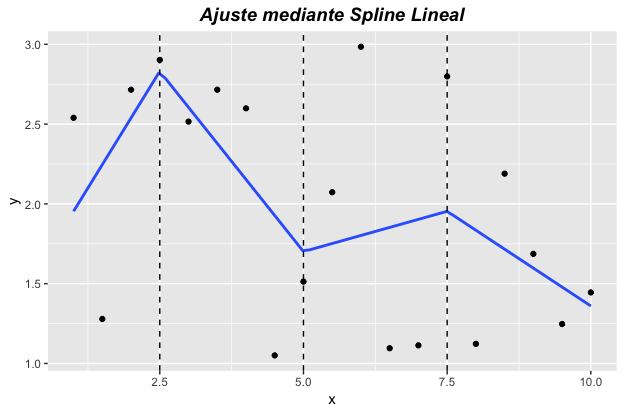
\includegraphics{images/spline_lineal.png}}
\caption{Spline Lineal.}
\label{spline_l}
\end{figure}




\vspace{0.5cm}

\hspace{0.4cm} Un spline de segundo grado es una uni\'on de polinomios cuadr\'aticos tal que $S(x)$ y su derivada $S^{(1)}(x)$ son continuas (ver figura \ref{spline_c}). Los polinomios $P(x)$ a trav\'es de los que construimos el Spline tienen grado 2. Esto quiere decir, que va a tener la forma $P(x) = ax^2 + bx + c$.

\hspace{0.4cm} Como en la interpolaci\'on segmentaria lineal, vamos a tener $N-1$ ecuaciones (donde N son los puntos sobre los que se define la funci\'on). La interpolaci\'on cuadr\'atica nos va a asegurar que la funci\'on que nosotros generemos a trozos con los distintos $P(x)$ va a ser continua, ya que para sacar las condiciones que ajusten el polinomio, vamos a determinar como condiciones,

\begin{itemize}
  \item Que las partes de la funci\'on a trozos P(x) pasen por ese punto. Es decir, que las dos Pn(x) que rodean al f(x) que queremos aproximar, sean igual a f(x) en cada uno de estos puntos.
  \item Que la derivada en un punto siempre coincida para ambos "lados" de la funci\'on definida a trozos que pasa por tal punto com\'un.
  \item Esto sin embargo no es suficiente, y necesitamos una condici\'on m\'as, la cual se obtiene a partir de una condici\'on de borde.
\end{itemize}




\hspace{0.4cm} Por su parte un spline c\'ubico, se representa mediante la uni\'on de polinomios c\'ubicos con primera y segunda derivada continuas (ver figura \ref{spline_3}). Este spline debido a su flexibilidad es el m\'as usado en las aplicaciones.

\vspace{0.5cm}

\begin{figure}[h]
  \scalebox{0.50}{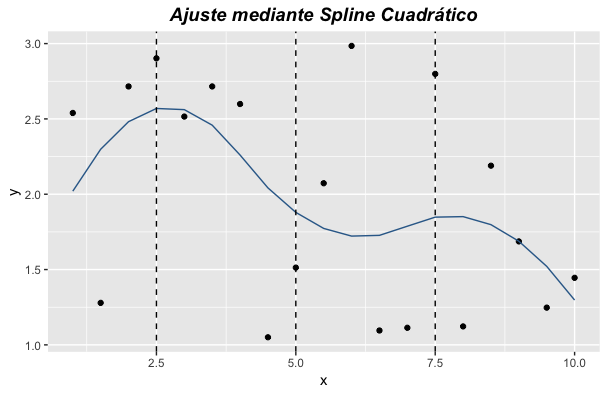
\includegraphics{images/spline_cuadratico.png}}
\caption{Spline Cuadr\'atico.}
\label{spline_c}
\end{figure}


\hspace{0.4cm}Formalmente un spline c\'ubico con nodos $x_{1},...x_{n}$ se define a partir de un conjunto de polinomios de la forma,\\

\begin{center}

$\displaystyle{S_{j}(x) = a_{j} + b_{j}x +c_{j}x^2 +d_{j}x^3}$
\end{center}


\vspace{0.5cm}

\noindent con $x_{j}<x<x_{j+1}$, sujeto a las siguientes condiciones,\\


\begin{center}

$\displaystyle{a_{j-1} + b_{j-1}x_{j} +c_{j-1}x_{j}^2 +d_{j-1}x_{j}^3 = a_{j} + b_{j}x_{j} +c_{j}x_{j}^2 +d_{j}x_{j}^3}$\\
$\displaystyle{ b_{j-1} +2c_{j-1}x_{j} +3d_{j-1}x_{j}^2 = b_{j} +2c_{j}x_{j} +3d_{j}x_{j}^2}$\\
$\displaystyle{ 2c_{j-1} +6d_{j-1}x_{j} = 2c_{j} +6d_{j}x_{j}}$\\
$\displaystyle{ c_{0} = d_{0} = c_{n} =d_{n}}$

\end{center}

\begin{figure}[h]
  \scalebox{0.50}{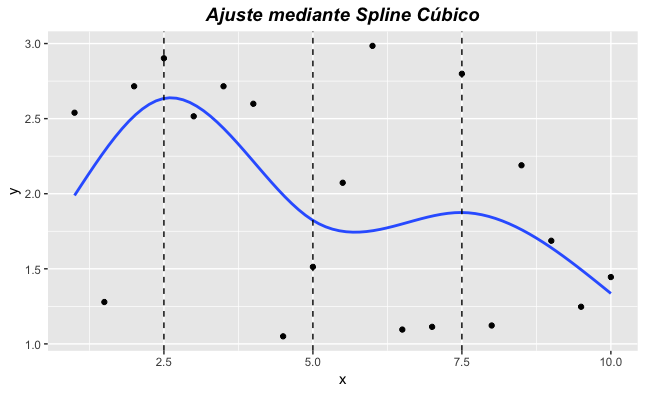
\includegraphics{images/spline_cubico.png}}
\caption{Spline C\'ubico.}
\label{spline_3}
\end{figure}


\hspace{0.4cm}As\'i para n nodos, existen $4(n-1)$ variables y $4(n-1)-2$ restricciones. Las mismas se deben a la necesidad de que el spline c\'ubico sea igual en los valores dados en cada nodo. Las primeras tres restricciones aseguran que la funci\'on resultante en su primera y segunda derivada sean continuas en los nodos. La restricci\'on final significa que el spline c\'ubico es lineal en el punto inicial y final de la muestra. Sin embargo, es importante resaltar que el spline c\'ubico tiene tercera derivada discontinua en los nodos.

\hspace{0.4cm}Debido a que hacen falta dos restricciones de borde, estas se deben a\~nadir. As\'i  $S^{(2)}(x_{1}) = S^{(2)}(x_{n}) = 0$ son las restricciones faltantes, estan hacen referencia a que el spline sea un spline c\'ubico natural. Como se mencion\'o al inicio si se considera una interpolaci\'on polinomial global de un conjunto de datos con mucho ruido pueden surgir aproximaciones no deseables e inestables. En constrate, un spline c\'ubico de interpolaci\'on encaja perfectamente con la suavidad de la funci\'on subyacente.

\begin{figure}[h]
  \scalebox{0.50}{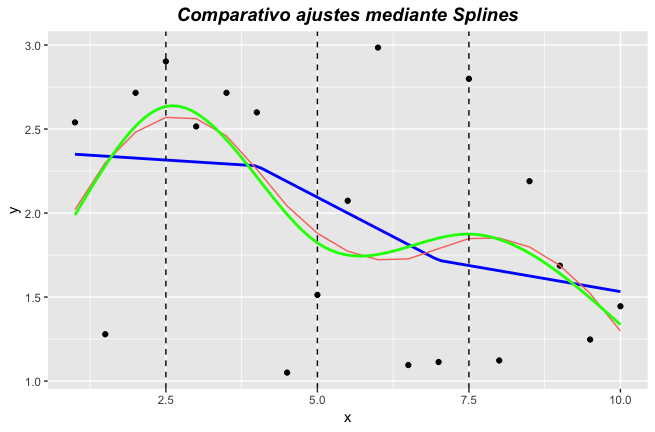
\includegraphics{images/Comparativo_splines.png}}
\caption{Comparativo Splines.}
\end{figure}

\vspace{0.5cm}

\hspace{0.4cm} Otra caracter\'istica de los splines es que con la adici\'on de un par\'ametro s\'olo se aumenta la dimensionalidad del espacio de par\'ametros en una unidad, ya que tres de los cuatro par\'ametros est\'an restringidos. De igual forma, al incrementar el n\'umero de nodos los splines toman formas funcionales m\'as flexibles, lo cual muestra la relaci\'on entre el grado aproximaci\'on que se logra con el spline y el n\'umero de nodos que lo definen.

\vspace{0.5cm}

\hspace{0.4cm} Mientras que las funciones spline son una herramienta interesante para interpolar funciones suaves, encontrarlas num\'ericamente no es tarea f\'acil. Una manera eficiente y muy estable para generar los splines necesarios para aproximar la funci\'on subyacente $f(x)$, es usando las bases de los B-splines c\'ubicos.

\vspace{0.5cm}

Bases de splines

\hspace{0.4cm} En el subcampo matem\'atico de an\'alisis num\'erico, una B-spline o Basis spline (o traducido una l\'inea polin\'omica suave b\'asica), es una funci\'on spline que tiene el m\'inimo soporte con respecto a un determinado grado, suavidad y partici\'on del dominio. Un teorema fundamental establece que cada funci\'on spline de un determinado grado, suavidad y partici\'on del dominio, se puede representar como una combinaci\'on lineal de B-splines del mismo grado y suavidad, y sobre la misma partici\'on. El t\'ermino B-spline fue propuesto por Isaac Jacob Schoenberg y es la abreviatura de spline b\'asica. Las B-splines pueden ser evaluadas de una manera num\'ericamente estable por el algoritmo de Boor. De un modo simplificado, se han creado variantes potencialmente m\'as r\'apidas que el algoritmo de Boor, pero adolecen comparativamente de una menor estabilidad.

\hspace{0.4cm} En el subcampo de la inform\'atica de dise\~no asistido por computadora y de gr\'aficos por computadora, el t\'ermino B-spline se refiere con frecuencia a una curva parametrizada por otras funciones spline, que se expresan como combinaciones lineales de B-splines (en el sentido matem\'atico anterior). Una B-spline es simplemente una generalizaci\'on de una curva de B\'ezier, que puede evitar el fen\'omeno Runge sin necesidad de aumentar el grado de la B-spline. Este fen\'omeno, se presenta al realizar interpolaci\'on lineal usando nodos equidistantes, b\'asicamente es un problema que se presenta con el error de aproximaci\'n en los extremos del intervalo que se este considerando, as\'i a medida que crece el n\'umero de nodos el error de aproximaci\'on se incrementa. 


\hspace{0.4cm} Supongamos que tenemos un conjunto infinito de nodos $...<x_{-2}<x_{-1}<x_{0}<x_{1}<x_{2}<...$, entonces el j-\'esimo B-spline de grado cero es igual a $B^{0}_{j}(x)=1$, si $x_{j} \leq x \leq x_{j+1}$ y $B^{0}_{j}(x)=0$ en otro caso. Con la funci\'on $B^{0}_{j}(x)$ como punto de partida se puede generar B-splines de grados mayores mediante la siguiente f\'ormula recursiva,\\

\begin{center}

$\displaystyle{B^{k}_{j}(x) = \frac{(x-x_{j})B^{k-1}_{j}(x)}{x_{j+k}-x_{j}} + \frac{(x_{j+k+1}-x)B^{k-1}_{j+1}(x)}{x_{j+k+1}-x_{j+1}}}$
\end{center}

\vspace{0.5cm}

\noindent para $k\geq 1$. As\'i un B-spline de grado $k$ se define como,\\

\begin{center}

$\displaystyle{S^{k}(x) = \sum_{j=-\infty}^{\infty} \theta^{k}_{j} B^{k}_{j-k}(x)}$
\end{center}

\vspace{0.5cm}

\hspace{0.4cm} Los coeficientes $\theta^{k}_{j}$ se llaman puntos de control o puntos de Boor. Hay $m-(n+1)$ puntos de control que forman una envoltura convexa.. Una buena interrogante ser\'ia el como se determina el valor de estos coeficientes en la expresi\'on anterior. Note que los B-splines de grado positivo no son ortogonales y por ende no poseen una expresi\'on simple para sus coeficientes.


Sin embargo, los c\'alculos empleados para los B-splines interpoladores de grado cero y uno, son bastante sencillos,\\

\begin{center}

$\displaystyle{S^{0}(x) = \sum_{j=-\infty}^{\infty} y_{j} B^{0}_{j}(x),\hspace{0.4cm} S^{1}(x) = \sum_{j=-\infty}^{\infty} y_{j} B^{1}_{j-1}(x) }$
\end{center}

\vspace{0.5cm}


\hspace{0.4cm} Cuando los nodos son equidistantes, la B-spline se dice que es uniforme, de otro modo ser\'a no uniforme. Si dos nodos tj son id\'enticos, cualquiera de las posibles formas indeterminadas 0/0 se consideran 0.


B-spline uniforme

\hspace{0.4cm} Cuando la B-spline es uniforme, las B-splines b\'asicas para un determinado grado n son s\'olo copias cambiadas de una a otra. Una alternativa no recursiva de la definici\'on de la B-splines $m-n+1$ b\'asica es,


\begin{center}
$\displaystyle{B_{j}^{n}(t)= B_{n}(t-t_{j}), \hspace{0.2cm}para \hspace{0.2cm}j=0,...,m-n-1 }$
\end{center}

\noindent con,

\begin{center}
$\displaystyle{B_{n}(t):= \frac{n+1}{n} \sum_{i=0}^{n+1}w_{i}^{n}(t - t_{i})_{+}^{n}   }$
\end{center}


\noindent donde,

\begin{center}
$\displaystyle{w_{i}^{n} := \prod_{j=0, j\neq i}^{n+1} \frac{1}{t_{j}- t_{i}}}$
\end{center}

\noindent n\'otese que $(t - t_{i})_{+}^{n}$ es la funci\'on potencia truncada definida como,

$$ (t - t_{i})_{+}^{n} := \left\{ % para la llave grandota
        \begin{tabular}{cc}
        	$0$ & si $t < t_{i}$ \\
        	$(t - t_{i})^{n}$ & si $t \ge t_{i}$ \\
        \end{tabular}
\right. $$


B-spline cardinal

\hspace{0.4cm} Si se define $B_{0}$ como la funci\'on caracter\'istica de ${\displaystyle [-{\tfrac {1}{2}},{\tfrac {1}{2}}]}$, y $B_{k}$ recursivamente como el producto convoluci\'on,


\begin{center}
$\displaystyle{B_{k} := B_{k-1}*B_{0}, \hspace{0.2cm} k=1,2,... }$
\end{center}

\noindent entonces $B_{k}$ se llaman B-splines cardinales (centradas). Esta definici\'on se remonta a Schoenberg. $B_{k}$ tiene soporte compacto ${\displaystyle [-{\tfrac {k+1}{2}},{\tfrac {k+1}{2}}]}$ y es una funci\'on impar. Como ${\displaystyle k\rightarrow \infty }$ las B-splines cardinales normalizadas tienden a la funci\'on de Gauss.

\hspace{0.4cm} Cuando el n\'umero de puntos de control de Boor es el mismo que el grado, la B-Spline degenera en una curva de B\'ezier. La forma de las funciones base es determinada por la posici\'on de los nodos. Escalar o trasladar el vector de nodo no altera las funciones de base.

\hspace{0.4cm} El spline est\'a contenido en el casco convexo de sus puntos de control. Una B-spline b\'asica de grado n $B_{i}^{n}(t)$ es distinta de cero s\'olo en el intervalo $[t_{i}, t_{i+n+1}]$ esto es,

$$ B_{i}^{n}(t) = \left\{ % para la llave grandota
        \begin{tabular}{cc}
        	$ > 0$ & si $t_{i}  \leq  t < t_{i+n+1}$ \\
        	$0$ & si $resto$ \\
        \end{tabular}
\right. $$

\hspace{0.4cm} En otras palabras si manipulamos un punto de control cambiamos s\'olo el comportamiento local de la curva y no el comportamiento global como con las curvas de B\'ezier. La funci\'on base se pueda obtener del polinomio de Bernstein. Algunos ejemplos de las bases B-splines se muestran acontinuaci\'on,

B-spline constante

\hspace{0.4cm} La B-spline constante es la spline m\'as simple. Se define en un solo tramo de nodo y ni siquiera es continua en los nodos. Es s\'olo la funci\'on indicador de los diferentes tramos de nodo.

$$ B_{j}^{0}(t) = 1_{[t_{j},t_{j+1})} = \left\{ % para la llave grandota
        \begin{tabular}{cc}
        	$ 1$ & si $t_{j}  \leq  t < t_{j+1}$ \\
        	$0$ & si $resto$ \\
        \end{tabular}
\right. $$



B-spline lineal

\hspace{0.4cm} La B-spline lineal se define en dos tramos de nodo consecutivos y es continua sobre los nodos, pero no diferenciable.

$$ B_{j}^{1}(t) = \left\{ % para la llave grandota
        \begin{tabular}{cc}
        	$\frac{t-t_{j}}{t_{j+1}-t_{j}} $ & si $t_{j}  \leq  t < t_{j+1}$ \\
        	$\frac{t_{j+2}-t}{t_{j+2}-t_{j+1}} $ & si $t_{j+1}  \leq  t < t_{j+2}$ \\
        	$0$ & si $resto$ \\
        \end{tabular}
\right. $$


B-spline cuadr\'atica uniforme

\hspace{0.4cm} Las B-splines cuadr\'aticas con nodo-vector uniforme es una forma com\'un de B-spline. La funci\'on base puede ser calculada f\'acilmente , y es igual para cada segmento, en este caso.

$$ B_{j}^{2}(t) = \left\{ % para la llave grandota
        \begin{tabular}{cc}
        	$\frac{1}{2} (1-t)^2$ \\
        	$-t^2+t+\frac{1}{2}$ \\
        	$\frac{1}{2} t^2$ \\
        \end{tabular}
\right. $$

\hspace{0.4cm} Escrito en forma de matriz, esto es,


\begin{center}
$\displaystyle{S_{i}(t) = \begin{bmatrix} t^2 & t & 1  \end{bmatrix} \frac{1}{2} \begin{bmatrix} 1 & -2 & 1\\ -2 & 2 & 0  \\ 1 & 1 & 0 \end{bmatrix} \begin{bmatrix}  \theta_{i-1} \\ \theta_{i} \\ \theta_{i+1}  \end{bmatrix} , \hspace{0.2cm} para \hspace{0.2cm} t \in [0,1],\hspace{0.2cm}  i=1,2,...,m-1 }$
\end{center}


B-spline c\'ubica

\hspace{0.4cm} Una formulaci\'on B-spline para un solo segmento puede ser escrita como,

\begin{center}
$\displaystyle{S_{i}(t) = \sum_{k=0}^{3} \theta_{i-3+k} B_{i-3+k}^{3}(t) \hspace{0.2cm} con \hspace{0.2cm} t \in [0,1]  }$
\end{center}


\noindent donde $S_{i}$ es el i-\'esimo segmento B-spline, $\theta$ es el conjunto de puntos de control, el segmento i y k es el \'indice del punto de control local y $ B_{i-3+k}^{3}(t)$ representa la base de B-spline de grado 3. Un conjunto de puntos de control $\theta$ ser\'ia  ${\displaystyle \theta_{i}^{w}=(w_{i}x_{i},w_{i}y_{i},w_{i}z_{i},w_{i})}$ donde el ${\displaystyle w_{i}}$ es el peso, tirando de la curva hacia el punto de control ${\displaystyle \theta_{i}}$ mientras que aumenta o se desplazan fuera de la curva, a la vez que disminuye.


\hspace{0.4cm} Toda una serie de segmentos se definir\'ia como,

\begin{center}
$\displaystyle{S(t) = \sum_{i=0}^{m-1} \theta_{i} B_{i}^{3}(t)  }$
\end{center}

\noindent donde i es el n\'umero de puntos de control y t es un par\'ametro global dados los valores de los nodos. Esta formulaci\'on expresa una curva B-spline como una combinaci\'on lineal de funciones B-spline b\'asicas, de ah\'i el nombre.

\hspace{0.4cm} Hay dos tipos de B-spline - uniforme y no uniforme. Una B-spline no uniforme es una curva donde los intervalos entre los puntos sucesivos de control no son, o no necesariamente son, iguales (el vector de nodos de espacios de nodo interiores no son iguales). Una forma com\'un es donde los intervalos se reducen sucesivamente a cero, interpolando los puntos de control.


B-spline c\'ubica uniforme

\hspace{0.4cm} La B-spline c\'ubica con vector-nodo uniforme es la forma m\'as usual de B-spline. La funci\'on base puede ser f\'acilmente calculada, y es igual para cada segmento, en este caso. Puesto en forma de matriz, esto es,


\begin{center}
$\displaystyle{S_{i}(t) = \begin{bmatrix} t^3  & t^2 & t & 1  \end{bmatrix} \frac{1}{6} \begin{bmatrix} -1 & 3 & -3 & 1 \\ 3 & -6 & 3 & 0 \\ -3 & 0 & 3 & 0 \\ 1 & 4 & 1 & 0 \end{bmatrix} \begin{bmatrix}  \theta_{i-1} \\ \theta_{i} \\ \theta_{i+1} \\ \theta_{i+2}  \end{bmatrix} , \hspace{0.2cm} para \hspace{0.2cm} t \in [0,1] }$
\end{center}





\hspace{0.4cm}Para splines de grados m\'as elevados, algunas arbitrariedades surgen al momento de calcular los coeficientes $\theta_{i}^{k}$. Por lo tanto, debido a que en las aplicaciones estadisticas existe un mayor inter\'es por encontrar una aproximaci\'on que una interpolaci\'on, la t\'ecnica de minimos cuadros puede ser empleada para calcular estos valores.


\vspace{0.5cm}

\hspace{0.4cm} Ahora bien, supongamos que se tiene un conjunto de $m$ funciones diferenciables $f(x)$, con soporte en el intervalo $[a,b]$, las cuales satifacen las siguientes condiciones,

% begin{itemize}
%   \item $f(x_{i})=y_{i}$, para i=1...,n
%   \item La m-1 derivada $f^{(m-1)}(x)$, es continua en x.
% \end{itemize}

\begin{itemize}
  \item[(i)] $f(x_{i})=y_{i}$, para $i=1...,n$.
  \item[(ii)] La m-1 derivada $f^{(m-1)}(x)$, es continua en x.
\end{itemize}

\hspace{0.4cm} El problema es encontrar entre todas esas funciones, una funci\'on tal que tenga la m\'inima integral del cuadro de su segunda derivada, esto es, una funci\'on que tenga el valor m\'as peque\~no de $\int_{a}^{b} (f^{(m)}(x))^2 dx$. Dicha funci\'on ser\'a la elecci\'on m\'as \'optima al momento de hallar un balance entre suavidad y ajuste de los datos.

\vspace{0.5cm}

\hspace{0.4cm} Se puede desmostrar que la soluci\'on de este problema es \'unica y la funci\'on en cuesti\'on es un spline polinomial que cumple la condici\'on i), y adem\'as satisface que,

\begin{itemize}
  \item[(a)] f es un pilinomio de grado no mayor que $m-1$ cuando $x \in [a,x_{1}]$ y $x \in [x_{n},b]$ .
  \item[(b)] F es un polinomio de grado no mayor a $2m-1$ para puntos interiores, $x \in [x_{i},x_{i+1}]$ con i=1,...,n.
  \item[(c)] f(x) tiene $2m-2$ derivadas continuas en el eje real.
\end{itemize}

\hspace{0.4cm} En resumen, la funci\'on $f$ m\'inima es un spline el cual est\'a conformado por trozos de polinomios unidos en los nodos $x_{i}$, donde dicha funci\'on tiene $2m-2$ derivadas continuas. N\'otese que en muchas aplicaciones $m=2$ es un valor muy utilizado y cuya soluci\'on viene dada mediante el spline c\'ubico natural.

\section{Regresi\'on no param\'etrica}

\hspace{0.4cm} La teor\'ia cl\'asica de la regresi\'on se basa, en gran parte, en el supuesto que las observaciones son independientes y se encuentran id\'entica y normalmente distribuidas. Si bien existen muchos fen\'omenos del mundo real que pueden modelarse de esta manera, para el tratamiento de ciertos problemas, la normalidad de los datos es insostenible. En el intento de eliminar esa restricci\'on se dise\~naron m\'etodos que hacen un n\'umero m\'inimo de supuestos sobre los modelos que describen las observaciones.

\hspace{0.4cm} La teor\'ia de los m\'etodos no param\'etricos trata, esencialmente, el desarrollo de procedimientos de inferencia estad\'istica, que no realizan una suposici\'on expl\'icita con respecto a la forma funcional de la 
distribuci\'on de probabilidad de las observaciones de la muestra. Si bien en la Estad\'istica no param\'etrica tambi\'en aparecen modelos y par\'ametros, ellos est\'an definidos de una manera m\'as general que en su contrapartida param\'etrica.

\hspace{0.4cm}La regresi\'on no param\'etrica es una colecci\'on de t\'ecnicas para el ajuste de funciones de regresi\'on cuando existe poco conocimiento a priori acerca de su forma. Proporciona funciones suavizadas de la relaci\'on y el procedimiento se denomina suavizado.

\hspace{0.4cm}Los fundamentos de los m\'etodos de suavizado son antiguos pero s\'olo lograron el estado actual de desarrollo gracias a los avances de la computaci\'on y los estudios por simulaci\'on han permitido evaluar sus comportamientos.

\hspace{0.4cm} La t\'ecnica m\'as simple de suavizado, los promedios m\'oviles, fue la primera en usarse, sin embargo han surgido nuevas t\'ecnicas como la estimaci\'on mediante n\'ucleos (``kernel") o la regresi\'on local ponderada. Estos estimadores de regresi\'on no param\'etrica son herramientas poderosas para el an\'alisis de datos, tanto como una t\'ecnica de estimaci\'on para resumir una relaci\'on compleja que no puede ser aprendida por un modelo param\'etrico, como para suplementar (o complementar) un an\'alisis de regresi\'on param\'etrico.

\hspace{0.4cm}En los an\'alisis param\'etricos se comienza haciendo supuestos r\'igidos sobre la estructura b\'asica de los datos, luego se estiman de la forma m\'as eficiente posible los par\'ametros que definen la estructura y por \'ultimo se comprueba si los supuestos iniciales se cumplen.

\hspace{0.4cm}La regresi\'on no param\'etrica, en cambio, desarrolla un ``modelo libre" para predecir la respuesta sobre el rango de valores de los datos. B\'asicamente est\'a constituida por m\'etodos que proporcionan una estimaci\'on suavizada de la relaci\'on para un conjunto de valores (de- nominado ventana) de la variable explicativa. Estos valores son ponderados de modo que, por ejemplo, los vecinos m\'as cercanos tengan mayor peso que los m\'as alejados dentro de una ventana de datos. Se pueden utilizar diversas funciones de ponderaci\'on, que son los pesos en que se basan los estimadores. La combinaci\'on de la funci\'on de ponderaci\'on y el ancho de la ventana inciden sobre la bondad de la estimaci\'on resultante.


\hspace{0.4cm} La mayor parte de las publicaciones sobre regresi\'on no param\'etrica consideran el caso de un solo regresor a pesar de que, a simple vista no pareciera de gran utilidad, ya que las aplicaciones m\'as interesantes involucran varias variables explicativas. Sin embargo, la regresi\'on no param\'etrica simple es importante por dos motivos:


\begin{itemize}
  \item En etapas preliminares del an\'alisis de datos o en pruebas de diagn\'ostico se utilizan gr\'aficos de dispersi\'on en los cuales puede ser muy \'util ajustar una ``curva suavizada". Por ejemplo, para explorar la forma de la funci\'on respuesta, para confirmar una funci\'on respuesta en particular que haya sido ajustada a los datos, para obtener estimaciones de la respuesta media sin especificar la forma de la funci\'on respuesta, para estudiar el cumplimientos de supuestos, etc.
  \item Forma la base a partir de la cual se extienden los conceptos para regresi\'on no param\'etrica m\'ultiple.
\end{itemize}


\section{Regresi\'on no param\'etrica mediante splines de suavizado.}

\hspace{0.4cm} Consideremos el siguiente modelo de regresi\'on homoced\'astico,\\

\begin{center}

$\displaystyle{Y_{i}=f(X_{i})+\epsilon_{i}}, \hspace{0.3cm} para \hspace{0.2cm} i=1,...,n$
\end{center}

\vspace{0.5cm}

\noindent donde los $\epsilon_{i}$ son errores de media cero independientes e id\'enticamente distribuidos.

\vspace{0.5cm}

\hspace{0.4cm} Uno de los posibles m\'etodos para emplear splines es aproximar la funci\'on de regresi\'on subyacente mediante las bases de splines, por ejemplo, la base de los B-splines c\'ubicos. As\'i, se escoge una secuencia fija de nodos $-\infty<t_{1}<t_{2}<...<t_{J}<\infty$, los cuales pueden diferir de los predictores. Luego, se calculan los elementos de la base c\'ubica de spline correspondiente.

\vspace{0.5cm}

\hspace{0.4cm}Es posible mostrar que s\'olo son necesarios $J+4$ elementos de esta base. Denotemos a estos elementos por $B_{j}(x)$, as\'i el spline polinomial lo podemos expresar como sigue,

\begin{center}

$\displaystyle{S(x)=\sum_{j=1}^{J+4} \theta_{j}B_{j}(x)}$
\end{center}

\vspace{0.5cm}

\hspace{0.4cm}Entonces los coeficientes $\theta_{j}$ pueden ser calculados al ser considerados como los par\'ametros que se obtienen al minimizar la suma de los errores al cuadrado,

 \begin{center}

$\displaystyle{\sum_{i=1}^{n} \left[ Y_{i} - \sum_{j=1}^{J+4} \theta_{j}B_{j}(X_{j})\right]^2}$
\end{center}

\vspace{0.5cm}

\hspace{0.4cm}Denotamos por $\hat{\theta_{j}}$ al estimador de m\'inimos cuadrados y definimos el estimador del spline polinomial como sigue,

 \begin{center}

$\displaystyle{ \hat{f}_{n}(x) = \sum_{j=1}^{J+4} \hat{\theta_{j}}B_{j}(x)}$
\end{center}

\vspace{0.5cm} Otro enfoque, se basa en la idea de encontrar un curva suave que minimize la suma penalizada de errores al cuadrado, es decir, que minimize la siguiente expresi\'on,

\begin{equation}\label{min}
  n^{-1}\sum_{j=1}^{n}(Y_{j}-f(X_{j}))^2+\mu \int_{a}^{b} [f^{(m)} (x)]^2 dx
\end{equation}

\vspace{0.5cm}


\noindent para alg\'un $\mu > 0$. As\'i como el enfoque de interpolaci\'on anterior, la soluci\'on de este problema de minimizaci\'on es un spline, el cual recibe el nombre de estimador de spline de suavizado.

\vspace{0.5cm}

\hspace{0.4cm} En particular, para el caso $m=2$ el minimizador de (\ref{min}), es un spline c\'ubico natural. Note que $\mu$ juega el papel de par\'ametro de suavizado, este t\'ermino se puede interpretar como una penalizaci\'on por rugosidad de la funci\'on. Curvas que cambian lenta o suavemente presentan un valor peque\~no de la integral, por ejemplo, en una funci\'on lineal la integral toma el valor de cero.

\vspace{0.5cm}

\hspace{0.4cm} De hecho, la primera suma en (\ref{min}) penaliza la falta de fidelidad de la aproximaci\'on de la data mediante el spline. El segundo t\'ermino es el responsable de la suavidad de la aproximaci\'on obtenida mediante el spline. Para ver esto consid\'erese los casos extremos, es decir, cuando $\mu =0$ y $\mu=\infty$. El primer caso conduce a una interpolaci\'on, esto es $\hat{f}(X_{i})=Y_{i}$ para $i=1,...,n$. El otro caso, conduce a una regresi\'on lineal pues $f^{(2)}(x)\equiv 0$.

\vspace{0.5cm}

\hspace{0.4cm} Por lo tanto $\mu$ es el par\'ametro de suavizado que controla la medida del estimador del spline polinomial, el cual puede variar desde el modelo m\'as complicado e inestable hasta el modelo m\'as simple. En otras palabras, la ecuaci\'on (\ref{min}) representa un balance entre la fidelidad o ajuste de los datos, representado mediante la suma de los residuos al cuadrado y la suavidad de la curva resultante, la cual se representa por la integral del cuadrado de la m-\'emisa derivada.


%Para citar un libro o un art\'{\i}culo se hace as\'{\i} : \cite{ADRS} \cite{Ar}


\chapter{Metodolog\'ia.}

\section{Elaboraci\'on de la base de datos.}


\hspace{0.4cm} La fuente principal de informaci\'on para calcular la curva de rendimientos para los t\'itulos de la deuda p\'ublica nacional es el Banco Central de Venezuela (BCV), el cual diariamente publica las operaciones realizadas con estos instrumentos y los publica en el documento ``resumersec"\hspace{0.01cm}  (Ver Figura \ref{doc_bcv}). Es importante destacar, que en este documento se encuentran por d\'ia dos pesta\~nas, la $``0-22"$ y la $``0-23"$, en la primera pesta\~na se encuentran las operaciones interbancarias, por su parte la segunda pesta\~na muestra informaci\'on sobre las operaciones realizadas por entes privados, en este caso el precio pautado en la operaci\'on no est\'a disponible, raz\'on por la cual esta pesta\~na no se toma en consideraci\'on. La informaci\'on disponible en la pesta\~na $``0-22"$ es la siguiente,

\begin{itemize}
  \item C\'odigo del instrumento: c\'odigo \'unico que se asocia a cada instrumento.
  \item Fecha de vencimiento: fecha de maduraci\'on de cada instrumento.
  \item Plazo: cantidad de d\'ias que faltan para que el instrumento venza.
  \item Cantidad de operaciones: n\'umero de operaciones realizadas con cada instrumento.
  \item Monto en Bol\'ivares: monto total involucrado en la operaci\'on.
  \item Precio m\'inimo: precio m\'as bajo pautado en la operaci\'on.
  \item Precio m\'aximo: precio m\'as alto pautado en la operaci\'on.
  \item Precio promedio: precio promedio pautado en la la operaci\'on. Cabe destacar que si existe una s\'ola operaci\'on, los precios m\'inimo, m\'aximo y promedio ser\'an iguales.
  \item Cup\'on: tasa de inter\'es pagadera por cada instrumento.
\end{itemize}


\vspace{0.5cm}

\begin{figure}[h]
  \scalebox{0.50}{\includegraphics{images/Imagen022.png}}
%\includegraphics[width=0.7\textwidth]{Imagen022.png}
\caption{Pesta\~na ``0-22".}
\label{doc_bcv}
\end{figure}

\vspace{0.5cm}

\hspace{0.4cm} Es importante recordar que dentro de los t\'itulos de la deuda p\'ublica nacional se encuentran los t\'itulos de inter\'es fijo (TIF) y los t\'itulos de tasa variable (VEBONO), los primeros se caracterizan por poseer una tasa de cup\'on que no varia, por su parte los VEBONO poseen una tasa de inter\'es variable.

\vspace{0.5cm}

\hspace{0.4cm}Esta informaci\'on tambi\'en es suministrada por el BCV, en su documento de las ``Caracter\'isticas de la deuda p\'ublica nacional" (Ver Figura \ref{doc_carac}), por lo cual el mismo se debe revisar con cierta frecuencia, con el fin de actualizar la tasa de cup\'on de los VEBONO. En este documento se muestra informaci\'on que caracteriza a cada instrumento, el mismo posee varias pesta\~nas, en este trabajo s\'olo se considerar\'a la pesta\~na $``DPN"$ en donde se encuentra informaci\'on sobre los instrumentos emitidos en moneda nacional. La informaci\'on disponible en este documento se muestra a continuaci\'on,

\begin{itemize}
  \item N\'umero-emisi\'on-decreto: informaci\'on sobre emisi\'on de cada instrumento.
  \item C\'odigo: c\'odigo \'unico que se asocia a cada instrumento.
  \item Fecha de emisi\'on: fecha cuando se emiti\'o cada instrumento.
  \item Fecha de vencimiento: fecha de maduraci\'on de cada instrumento.
  \item Monto en circulaci\'on: monto total de cada instrumento en circulaci\'on.
  \item Porcentaje de referecia: indica si el instrumento es de tasa fija o tasa variable.
  \item Fecha de inicio: indica cada cuanto tiempo el instrumento paga cup\'on.
  \item Per\'iodo vigente: indica el per\'iodo (fecha inicio y fecha fin) cuando cada instrumento paga cup\'on.
  \item Tasa: cup\'on asociado a cada instrumento.
\end{itemize}



\begin{figure}[h]
  \scalebox{0.50}{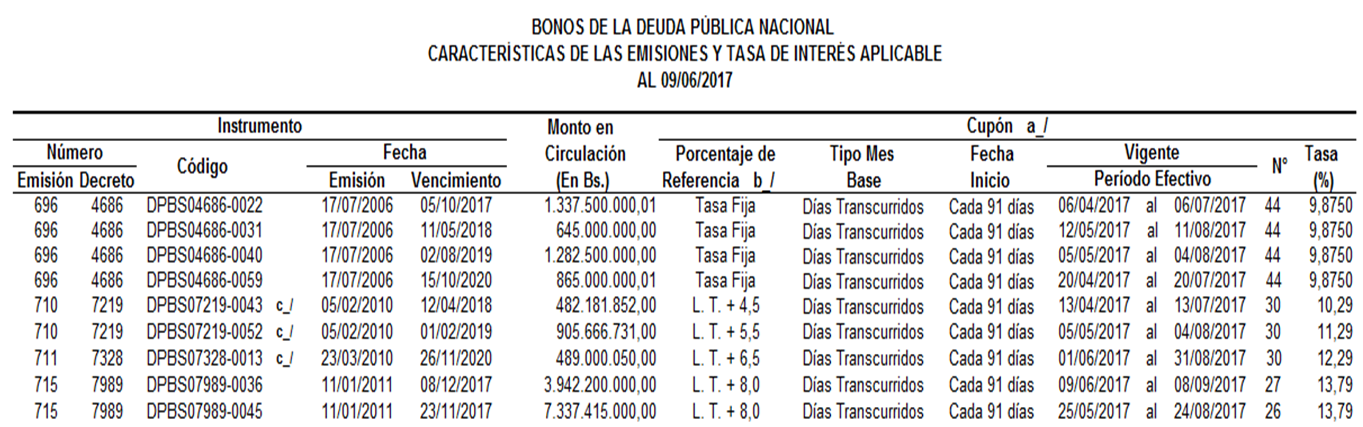
\includegraphics{images/Imagencarac.png}}
\caption{Caracter\'isticas.}
\label{doc_carac}
\end{figure}


\hspace{0.4cm} A partir de la pesta\~na ``0-22"\hspace{0.01cm} y del documento de las caracter\'isticas, se cre\'o la base de datos con la cual se va a trabajar, la misma contiene no s\'olo la informaci\'on suministrada por la pesta\~na ``0-22", sino alguna informaci\'on adicional tomada del documento de las caracter\'isticas. En dicha base de datos se contar\'a con la siguiente informaci\'on,

\vspace{0.5cm}

\begin{itemize}
  \item Tipo instrumento: indica el tipo de instrumento.
  \item Nombre: proporciona el nombre corto del t\'itulo, usualmente este nombre se conforma por el tipo de t\'itulo m\'as su mes y a\~no de vencimiento, por ejemplo, el t\'itulo TIF032028, representa al t\'itulo TIF con vencimiento en marzo del 2028.
  \item Fecha de operaci\'on: indica la fecha en que se efectu\'o dicha operaci\'on.
  \item Fuente: indica la fuente de donde se tom\'o la informaci\'on, esta se puede tomar de dos fuentes, la primera mediante la pesta\~na 0-22 (mercado secundario) y  la otra mediante el documento de las subastas (mercado primario, informaci\'on suministrada por el BCV).
  \item Sicet: proporciona el c\'odigo asociado a cada t\'itulo.
  \item Fecha de vencimiento: indica la fecha de maduraci\'on (vencimiento) del instrumento.
  \item Plazo: indica la cantidad de d\'ias que falta para que el instrumento se venza.
  \item Cantidad de operaciones: proporciona la cantidad de operaciones efectuadas con un insrumento en espec\'ifico.
  \item Monto: indica el monto en Bol\'ivares, por el cual se efectu\'o la operaci\'on u operaciones.
  \item Precio m\'inimo: indica el precio m\'inimo, por el cual se trans\'o la operaci\'on.
  \item Precio m\'aximo: indica el precio m\'aximo, por el cual se trans\'o la operaci\'on.
  \item Precio promedio: indica el precio promedio, por el cual se trans\'o la operaci\'on, cabe destacar que en dado caso de existir una sola operaci\'on el valor del precio m\'inimo, m\'aximo y promedio van a coincidir.
  \item Cup\'on: proporciona la tasa de cup\'on asociado a cada instrumento.
  \item Frecuencia: indica con que frecuencia el instrumento paga cup\'on, para los TIF y VEBONO, esta es 4, pues los mismos pagan cu\'pon trimestralmente, as\'i se obtiene este valor pues existen 4 trimestres en el a\~no.

\end{itemize}

\vspace{0.5cm}

\hspace{0.4cm} Una vez obtenida la base de datos esta seg\'un sea el caso puede ser depurada mediante ciertos criterios, el primero es que aquellas operaciones con un monto menor a los 10 milllones no se consideran. El segundo es considerar la operaci\'on mas reciente, es decir, si en la base de datos se tiene que para un mismo instrumento existen diferentes operaciones en diferentes d\'ias, s\'olo se considerar\'a la operaci\'on m\'as reciente.

%El segundo es el tipo de fuente, siempre prevalecer\'a la fuente subasta.

\hspace{0.4cm} Para efectuar la depuraci\'on, a la base de datos anterior se le a\~nadir\'an dos columnas nuevas una que indica el rendimiento al vencimiento de cada instrumento y la otra que indica la decisi\'on que se tom\'o en base a los criterios descritos anteriormente (Ver Figura \ref{base_datos}). Esta \'ultima ser\'a una variable dicot\'omica, es decir solo con dos valores (0 \'o 1), en donde ``0" me indica que no selecciono el t\'itulo y ``1" me indica que si lo tomo en cuenta para el estudio a realizar.

\begin{figure}[h]
  \scalebox{0.50}{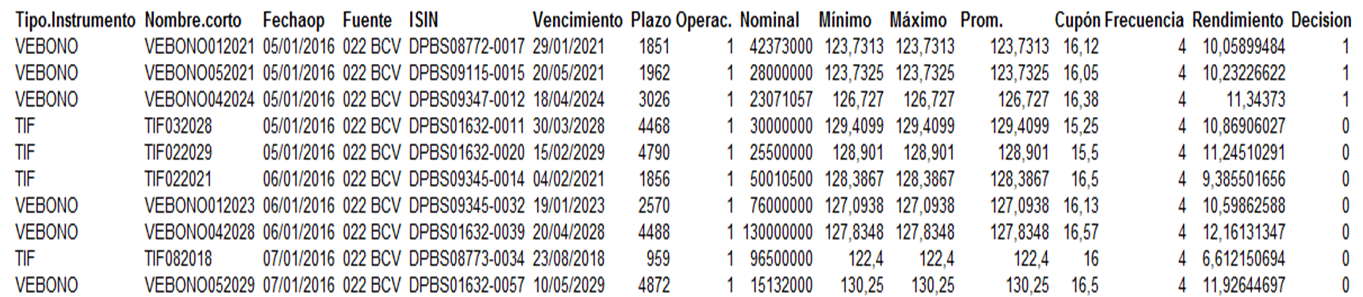
\includegraphics{images/Imagenbase.png}}
\caption{Base de datos.}
\label{base_datos}
\end{figure}


\hspace{0.4cm} Una vez calculados los precios estimados asociados a cada instrumento, se proceder\'a a comparar los mismo con aquellos obtenidos por una metodolog\'ia distinta. La metodolog\'ia con la cual se va a comparar es la de Svensson, la cual es una metodolog\'ia param\'etrica.



\hspace{0.4cm} Los instrumentos a considerar ser\'an aquellos pertencientes al portafolio de inversiones de una instituci\'on financiera, de tal manera que para un d\'ia especifico sea posible conocer cuanta es la ganancia o p\'erdida que generan estos instrumentos. y por ende saber si es viable la venta o compra de determinado instrumento.


\hspace{0.4cm} A partir de la data obtenida (Ver Figura \ref{base_datos}), se proceder\'a a a\~nadir unas columnas nuevas con el fin de clasificar las observaciones para los distintos instrumentos en diferentes per\'iodos de vencimiento. Los per\'iodos de vencimiento son,

\begin{itemize}
\item Corto plazo: se refiere al vencimiento m\'as cercano, los instrumentos que se encuentran aqu\'i son aquellos que poseen un vencimiento menor a un a\~no.
\item Mediano plazo: en esta clasificaci\'on se encuentran los instrumentos cuyo vencimiento este entre uno y diez a\~nos.
\item Largo plazo: hace referencia a aquellos instrumentos que tengan un vencimiento mayor a diez a\~nos.
\end{itemize}

\hspace{0.4cm} Luego de separar la data por tipo de instrumento, la nueva data con la que se trabajar\'a es la siguiente,

\begin{figure}[h]
  \scalebox{0.50}{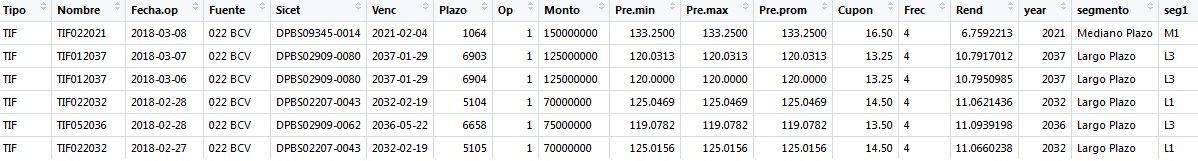
\includegraphics{images/data_nueva.png}}
\caption{Base de datos TIF.}
\label{base_datos_tif}
\end{figure}

\hspace{0.4cm} Con el fin de contar con la data m\'as reciente a partir de la fecha de valoraci\'on, se cre\'o la funci\'on ``extrae" \hspace{0.01cm} la cual selecciona de la data de la Figura (\ref{base_datos_tif}) una determinada cantidad de observaciones, la cual es especificada por el usuario, esta funci\'on cuenta con los siguientes argumentos,

\begin{itemize}
 \item fv: indica la fecha de valoraci\'on para la cual se est\'a realizando el estudio.
 \item dias: indica la cantidad de d\'ias que el usuario desea, a partir de este valor se va a obtener la data con la que se va a trabajar.
 \item data: hace referencia a la data completa para cada tipo de instrumento, a partir de la misma se procedera a extraer parte de ella a partir del n\'umero de dias seleccionado.
\end{itemize}

\hspace{0.4cm} Luego de selecionar la data, la misma se procede a depurar, es decir, se van a eliminar las observaciones duplicadas considerando s\'olo aquellas que sean m\'as recientes. 


\hspace{0.4cm}As\'i a partir de esta data s\'olo se consideraran las columnas plazo y rendimiento con el fin de tener una nube de puntos a partir de la cual se haga el ajuste de la funci\'on spline, y as\'i obtener la curva de rendimientos.

\newpage

\hspace{0.4cm} La data obtenida a partir de la depuraci\'on anterior es,

\begin{figure}[h]
    {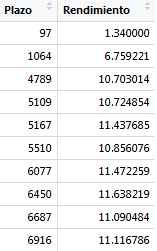
\includegraphics{images/cand.png}}
\caption{Data depurada TIF.}
\label{fig91}
\end{figure}



\hspace{0.4cm} Una vez obtenida la data para los Tif y Vebono se utiliz\'o la funci\'on ``smooth.spline" \hspace{0.01cm} del programa estad\'istico R, para ajustar un spline c\'ubico a la data ingresada. Los argumentos requeridos por esta funci\'on son los siguientes,

\begin{itemize}
  \item X: representa el vector de la variable predictiva.
  \item Y: representa el vector de la variable repuesta.
  \item cv: (TRUE/FALSE) variable del tipo l\'ogico que representa si se va a utilizar la validaci\'on cruzada generalizada al momento de calcular el par\'ametro de suavizamiento.
  \item Spar: representa el par\'ametro de suavizamiento, t\'ipicamente (aunque no necesariamente) ubicado entre 0 y 1. Es el coeficiente lambda que acompa\~na a la integral del cuadrado de la segunda derivada de la funci\'on f.
\end{itemize}

\hspace{0.4cm} De esta manera el siguiente comando ajusta un spline cubico a la data ingresada,


spline1=smooth.spline(X=datT1\$Plazo,Y=datT1\$Rendimiento,cv=TRUE, spar=1.35)


\noindent y lo guarda en la variable ``spline1".

\hspace{0.4cm} Es importante se\~nalar lo crucial de la escogencia del par\'ametro ``spar", pues de \'el depende que tan suave sea la curva, la Figura \ref{comp_spar} muestra como var\'ia la curva cuando se cambia  el valor del ``spar", para esta comparaci\'on se us\'o tres valores, el primero fue 0.51 con el cual se obtiene una curva con ciertos picos la cual no es suave en lo absoluto. 

\newpage

\hspace{0.4cm} Usando el valor de 0.71 se obtiene la curva roja la cual presenta una mayor suavidad. Mientras que usando el valor de 0.81 se obtiene un mejor resultado aunque similar al anterior. De esta manera, se puede observar la importancia de la elecci\'on correcta de este par\'ametro, mientras este valor se aproxime a 1 se obtendr\'a una curva con mayor suvidad.

\begin{figure}[h]
  {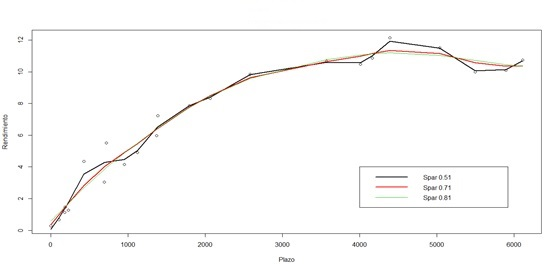
\includegraphics{images/curvavbv2.jpg}}
\caption{Curva de rendimiento Vebono para diferentes valores de suavizado.}
\label{comp_spar}
\end{figure}

\hspace{0.4cm} Cabe destacar que para cada versi\'on el par\'ametro usado en la variable ``spar" \hspace{0.2cm} cambi\'o. Esto debido a la diferente cantidad de puntos que tiene cada versi\'on. As\'i el valor del par\'ametro ``spar" \hspace{0.2cm} para los TIF se ubic\'o en el siguiente intervalo [0.4,0.6], por su parte para los VEBONOS la elecci\'on de dicho par\'ametro esta en [0.3,0.5]. Los mismos se obtuvieron mediante ensayo y error. Para los valores ubicados dentro de los intervalos mencionados siempre se obtuvo una curva suave.

\hspace{0.4cm} Una vez que se obtiene la curva estimada y es guardada en una variable (en este caso, la variable es spline1), se procede a aplicar el comando ``predict", para estimar el rendimiento de alg\'un plazo que se ingrese.

\hspace{0.4cm} As\'i con el fin de calcular el precio estimado de cada t\'itulo, se cre\'o la funci\'on ``precio"\hspace{0.01cm} mediante R, para determinar de forma autom\'atica dichos valores. Los imputs de dicha funci\'on son los siguientes,


\begin{itemize}
  \item Tit: representa el nombre de cada t\'itulo, al cual se le quiere estimar su precio, el mismo debe ser un car\'acter, ej: TIF102017 \'o VEBONO112017.
  \item Spline1: representa la variable donde se guardo la curva ajustada mediante el spline.
  \item Fv: indica la fecha de valoraci\'on, para la cual se desea conocer el precio estimado.
\end{itemize}


\hspace{0.4cm} Una vez ingresado los imputs, la funci\'on internamente busca el nombre del t\'itulo en el documento de las caracter\'isticas m\'as reciente, y extrae del mismo la fecha de pago del pr\'oximo cup\'on y su fecha de vencimiento, con el fin de crear un vector de flujos.


\hspace{0.4cm} Por ejemplo, si se quiere conocer el precio estimado del t\'itulo ``TIF032022" \hspace{0.01cm} al ``01/03/2018", la funci\'on busca su fecha de vencimiento $(03/03/2022)$ y la fecha de pago del pr\'oximo cup\'on la cual es en este caso $08/03/2018$. Luego con dichos valores calcula la Tabla \ref{tabla1}, que representa los cupones que le quedan por pagar al t\'itulo,

\renewcommand{\tablename}{Tabla}
\begin{table}[H]
\centering
%\begin{center}
{\begin{tabular}[t]{|l |c |c |c |c |c |r|}
\hline
Fecha & Plazo t\'itulo & Plazo a\~nos & Rend estimado & Exp & Cup\'on & Producto \\
\hline
08/03/2018 & 7  & 0,0191780 & 0,45\% & 0,9999131 & 4& 3,999652\\
\hline
07/06/2018 & 98 & 0,2684931 & 1,05\% & 0,9971804 & 4& 3,988721\\
\hline
06/09/2018 & 189 & 0,5178082 & 1,64\% & 0,9915025 & 4& 3,966010\\
\hline
06/12/2018 & 280 & 0,7671232 & 2,23\% & 0,9829646 & 4& 3,931859\\
\hline
07/03/2019 & 317 & 1,0164383 & 2,82\% & 0,9717013 & 4& 3,886805\\
\hline
06/06/2019 & 462 & 1,2657534 & 3,39\% & 0,9578928 & 4& 3,831571\\
\hline
05/09/2019 & 553 & 1,5150684 & 3,96\% & 0,9417596 & 4& 3,767038\\
\hline
05/12/2019 & 644 & 1,7643835 & 4,50\% & 0,9235567 & 4& 3,694227\\
\hline
05/03/2020 & 735 & 2,0136986 & 5,03\% & 0,9035668 & 4& 3,614267\\
\hline
04/06/2020 & 826 & 2,2630137 & 5,54\% & 0,8820934 & 4& 3,528373\\
\hline
03/09/2020 & 917 & 2,5123287 & 6,02\% & 0,8594532 & 4& 3,437813\\
\hline
03/12/2020 & 1008 & 2,7616438 & 6,48\% & 0,8359698 & 4& 3,343879\\
\hline
04/03/2021 & 1099 & 3,0109589 & 6,91\% & 0,8119665 & 4& 3,247866\\
\hline
03/06/2021 & 1190 & 3,2602739 & 7,31\% & 0,7877226 & 4& 3,150890\\
\hline
02/09/2021 & 1281 & 3,5095890 & 7,69\% & 0,7634473 & 4& 3,053789\\
\hline
02/12/2021 & 1372 & 3,7589041 & 8,03\% & 0,7393192 & 4& 2,957277\\
\hline
03/03/2022 & 1463 & 4,0082191 & 8,35\% & 0,7154912 & 104 & 74,411084\\
\hline
% Precio &  &  &  & & & 112,688809\\
\multicolumn{6}{|c|}{Precio} & 131,8111 \\
\hline
\end{tabular}
}
%\caption{Tabla}
%\end{center}
\caption{C\'alculos funci\'on precio.}
\label{tabla1}
\end{table}

\hspace{0.4cm}As\'i la primera columna (Fecha) se obtiene de sumarle a la fecha de pago del pr\'oximo cup\'on ($08/03/2018$) 91 d\'ias, que representa el tiempo cada cuando el t\'itulo paga cup\'on, esto se realiza  hasta llegar a la fecha de vencimiento.

\hspace{0.4cm} Luego la columna ``Plazo t\'itulo", se obtiene realizando la diferencia entre la columna 1 y la fecha de valoraci\'on (01/03/2018). Luego la columna 3 se obtiene dividiendo el valor de la columna 2 entre 365, para pasar dicho valor a a\~nos. Despu\'es eval\'uo los valores de la columna 2 en el spline obtenido, para as\'i obtener los rendimientos estimados (columna 4). Posteriormente en la columna 5 (EXP) calculo la exponencial del producto de menos uno con el plazo en a\~nos (columna 3) y con el rendimiento estimado (columna 4).


\hspace{0.4cm} La columna 6 (Cup\'on) la calculo dividiendo el valor del cup\'on del t\'itulo entre 4, ya que cada cup\'on se paga cada tres meses, a diferencia del \'ultimo al cual se le debe sumar el valor de 100. Finalmente en la \'ultima columna (Producto) calculo el producto del valor de la columna EXP con la columna Cup\'on, para luego realizar la sumatoria de todas sus filas y as\'i obtener el precio estimado ( 131,8111 en este caso).


\hspace{0.4cm}El mismo procedimiento se repite para cada t\'itulo ya sea Tif o Vebono. Es importante se\~nalar que los t\'itulos considerados fueron aquellos que pertenec\'ian al portafolio de inversiones del banco en un tiempo determinado.

\section{Estimaci\'on de par\'ametros y curva de rendimiento.}

\hspace{0.4cm} Una vez construida la base de datos, se proceder\'a a utilizar los splines de suavizado para obtener los par\'ametros necesarios para la curva de rendimientos. Recordemos que esta curva relaciona el plazo del instrumento con su rendimiento.


\hspace{0.4cm} Es importante se\~nalar que se estimar\'a una curva por cada tipo de instrumento, as\'i se obtendr\'a un curva para los TIF y una curva para los VEBONO. Por tal raz\'on a partir de la base de datos, se separar\'a los TIF de los VEBONOS, y se considerar\'an s\'olo las columnas Plazo y Rendimiento para estimar dicha curva. Seg\'un sea el caso, s\'olo considerar\'an aquellas observaciones que tengan decisi\'on 1.


\hspace{0.4cm} Aunado a cada tipo de instrumento (TIF \'o VEBONO), se considerar\'a un instrumento de otro tipo este es la letra del tesoro, este tipo de instrumento representar\'a el punto inicial la curva, cabe destacar que la letra a considerar debe ser aquella cuya fecha de operaci\'on sea la m\'as reciente con respecto a la fecha de valoraci\'on (d\'ia en que se quiere conocer los rendimientos estimados).


\hspace{0.4cm} A partir de la curva de rendimientos obtenida (Ver Figura \ref{c_rend}) es posible calcular un rendimiento estimado para alg\'un tipo de instrumento a partir de su plazo, que no es m\'as que la cantidad de d\'ias que faltan por transcurrir hasta su vencimiento. Este valor es de suma importancia ya que a partir del mismo es posible calcular el precio estimado asociado a cada instrumento en un d\'ia espec\'ifico. Con lo cual es posible saber a partir de la historia (base de datos), el precio estimado de alg\'un instrumento que le interese a cierta instituci\'on y por ende saber si ese t\'itulo es rentable o no, es decir, si vale la pena invertir en el mismo o no.

\begin{figure}[h]
  \scalebox{0.40}{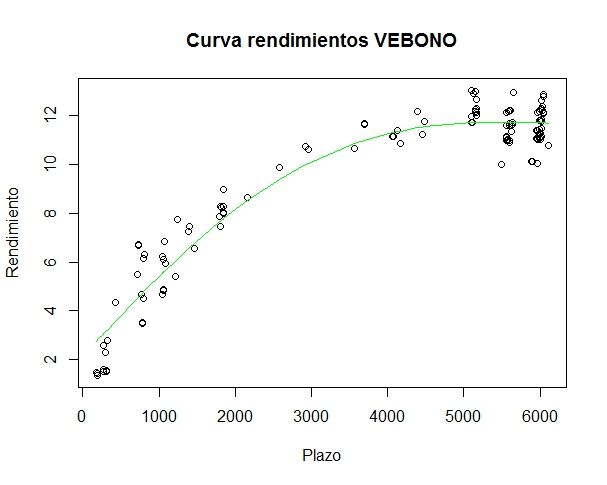
\includegraphics{images/curvarend.jpeg}}
\caption{Curva de rendimiento.}
\label{c_rend}
\end{figure}

\hspace{0.4cm} Como se dijo anteriormente, los resultados de los precios obtenidos mediante el uso de la metodolog\'ia de splines de suavizado ser\'an comparados con los precios obtenidos a trav\'es de la metodolog\'ia de Svensson. En dicha metodolog\'ia existe un proceso de optimizaci\'on el cual permite encontrar los par\'ametros id\'oneos, de tal manera que la diferencia entre los precios promedio de cada instrumento y su precio te\'orico sea lo m\'as peque\~na posible. El proceso de esta optimizaci\'on se muestra a continuaci\'on.


%\section{Elecci\'on \'optima del par\'ametro de suavizamiento.}

\newpage

\section{Proceso de optimizaci\'on de Svensson.}


\hspace{0.4cm} Para aplicar este proceso es necesario tener una funci\'on objetivo, sobre la cual se realizar\'a el proceso de optimizaci\'on, ya sea para maximizar \'o minimizar dicha funci\'on. Dependiendo de la forma de dicha funci\'on el proceso de optimizaci\'on ser\'a lineal o no lineal. En nuestro caso particular se llevar\'a a cabo un proceso de optimizaci\'on no lineal donde se buscar\'a minimizar la funci\'on objetivo.


\hspace{0.4cm} En el c\'alculo de nuestra funci\'on objetivo inteviene el concepto de la duraci\'on de un bono \'o t\'itulo, la cu\'al es una medida del vencimiento medio ponderado de todos los flujos que paga un bono. La misma viene dada mediante la siguiente expresi\'on, \\

\begin{center}

$\displaystyle{Duracion = \frac{1+r}{r} - \frac{n(c-r)+(1+r)}{c(1+r)^{n}-(c-r)}}$

\end{center}


\noindent donde

\begin{itemize}
  \item r es el rendimiento al vencimiento del bono durante el per\'iodo considerado.
  \item n es el n\'umero de per\'iodos que restan hasta la fecha de vencimiento del bono.
  \item c es el cup\'on del bono.
\end{itemize}


\hspace{0.4cm} As\'i nuestra funci\'on objetivo viene dada mediante la siguiente expresi\'on,

\vspace{0.2cm}

\begin{equation}\label{ecua2}
  f(x) = \sum_{i=1}^{n} (w_{i}\epsilon(x)_{i} )^2
\end{equation}


\noindent donde $w_{i}$ representan las ponderaciones, y se calculan mediante la siguiente expresi\'on,

\vspace{0.2cm}


\begin{center}

$\displaystyle{w_{i} = \frac{\frac{1}{D_{i}}}{\sum_{j=1}^{N}\frac{1}{D_{j}}}}$

\end{center}


\vspace{0.2cm}


\noindent por su parte, $\epsilon_{i}(x)= \hat{Pr}_{i}(x)-Pr_{i}$, donde $Pr_{i}$ representan los precios promedios de los t\'itulos a considerar, de entrada este es un par\'ametro \'o valor con el que se cuenta. Por otra parte $\hat{Pr}_{i}(x)$ representa los precios estimados donde $x$ es el par\'ametro que va a variar y es el valor que se quiere optimizar.


\hspace{0.4cm} Mediante la funci\'on objetivo descrita anteriormente se busca minimizar la diferencia que existe entre los precios promedios y los precios estimados, calculando un valor \'optimo del par\'ametro $x$ mediante el proceso de optimizaci\'on no lineal.



\hspace{0.4cm}El proceso de optimizaci\'on se realiz\'o mediante el software estad\'istico R, mediante el paquete ``nloptr". En este paquete, se encuentra el comando ``aulag" el cual minimiza un funci\'on objetivo y devuelve entre otros valores el par\'ametro m\'as \'optimo, que hace que la funci\'on sea m\'inima. Un ejemplo del uso de este comando se presenta acontinuaci\'on,

\begin{center}
  $ala2=auglag(1.22, fn=mifuncion, hin=res)$
\end{center}


\noindent donde el primer argumento debe ser el valor inicial del par\'ametro a optimizar, el segundo argumento ``fn" se refiere a la funci\'on que se desea optimizar, finalmente en el tercer par\'ametro ``hin" se indican las restricciones sobre el par\'ametro a optimizar, en este caso la restricci\'on establecida es que el par\'ametro sea mayor a cero.


\hspace{0.4cm} Recordemos que la tasa cero cup\'on que se obtiene mediante la metodolog\'ia de Svensson est\'a dada por la siguiente expresi\'on,\\


$\displaystyle{s(m) = \beta_{0}+ \beta_{1}\frac{\left(1-e^\frac{-m}{\tau_{1}}\right)}{m/\tau_{1}} + \beta_{2} \left(\frac{\left(1-e^\frac{-m}{\tau_{1}}\right)}{m/\tau_{1}} -  e^\frac{-m}{\tau_{1}}\right) + \beta_{3} \left(\frac{\left(1-e^\frac{-m}{\tau_{2}}\right)}{m/\tau_{2}} -  e^\frac{-m}{\tau_{2}}\right)}$\\

\noindent esta expresi\'on est\'a sujeta a las siguientes restricciones,

\begin{itemize}
  \item $\beta_{0} > 0$
  \item $\beta_{0}+\beta_{1} > 0$
  \item $\tau_{1} > 0$
  \item $\tau_{2} > 0$
\end{itemize}

\noindent cada par\'ametro controla una secci\'on de la curva. La f\'ormula anterior es de suma importancia ya que ella interviene en el c\'alculo del precio te\'orico de cada instrumento. El proceso de optimizaci\'on act\'ua directamente sobre esta f\'ormula, ya que el mismo se centra en variar los par\'ametros de tal manera que la funci\'on objetivo sea minimizada.

\hspace{0.4cm} Como se observ\'o en las secciones anteriores el par\'ametro de suavizamiento fu\'e elegido mediante el m\'etodo de ensayo y error el cual no es para nada \'optimo pues a priori este m\'etodo no nos garantiza que el valor seleccionado sea el mejor, ya que se contar\'ian con una gran cantidad de posibles valores a seleccionar, con el fin  de encontrar dicho par\'ametro el procedimiento anteriormente explicado puede ser implementado. 

\hspace{0.4cm} Sin embargo, al realizar este proceso, se obtienen curvas que no son para nada suaves y en ocasiones no poseen ningunas de las formas usuales de la curva de rendimientos. Esto es debido a que en este caso este proceso, var\'ia el par\'ametro de suavizamiento de tal manera que la diferencia entre el precio promedio y el precio te\'orico sea lo mas peque\~na posible y en este proceso no existe un par\'ametro que controle la forma de la curva obtenida. Por lo tanto, su aplicaci\'on presenta algunos inconvenientes.  







\chapter{Resultados y conclusiones.}




\section{Estimaci\'on de par\'ametros y curva de rendimiento.}

\hspace{0.4cm} Una vez construida la base de datos, se proceder\'a a utilizar los splines de suavizado para obtener los par\'ametros necesarios para la curva de rendimientos. Recordemos que esta curva relaciona el plazo del instrumento con su rendimiento.


\hspace{0.4cm} Es importante se\~nalar que se estimar\'a una curva por cada tipo de instrumento, as\'i se obtendr\'a un curva para los TIF y una curva para los VEBONO. Por tal raz\'on a partir de la base de datos, se separar\'a los TIF de los VEBONOS, y se considerar\'an s\'olo las columnas Plazo y Rendimiento para estimar dicha curva. Seg\'un sea el caso, s\'olo considerar\'an aquellas observaciones que tengan decisi\'on 1.


\hspace{0.4cm} Aunado a cada tipo de instrumento (TIF \'o VEBONO), se considerar\'a un instrumento de otro tipo este es la letra del tesoro, este tipo de instrumento representar\'a el punto inicial la curva, cabe destacar que la letra a considerar debe ser aquella cuya fecha de operaci\'on sea la m\'as reciente con respecto a la fecha de valoraci\'on (d\'ia en que se quiere conocer los rendimientos estimados).


\hspace{0.4cm} A partir de la curva de rendimientos obtenida (Ver figura \ref{c_rend}) es posible calcular un rendimiento estimado para alg\'un tipo de instrumento a partir de su plazo, que no es m\'as que la cantidad de d\'ias que faltan por transcurrir hasta su vencimiento. Este valor es de suma importancia ya que a partir del mismo es posible calcular el precio estimado asociado a cada instrumento en un d\'ia espec\'ifico. Con lo cual es posible saber a partir de la historia (base de datos), el precio estimado de alg\'un instrumento que le interese a cierta instituci\'on y por ende saber si ese t\'itulo es rentable o no, es decir, si vale la pena invertir en el mismo o no.

\begin{figure}[h]
  \scalebox{0.40}{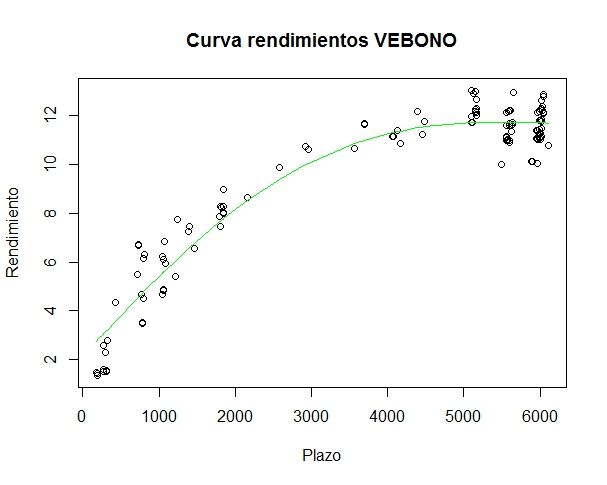
\includegraphics{images/curvarend.jpeg}}
\caption{Curva de Rendimiento.}
\label{c_rend}
\end{figure}

\hspace{0.4cm} Como se dijo anteriormente, los resultados de los precios obtenidos mediante el uso de la metodolog\'ia de splines de suavizado ser\'an comparados con los precios obtenidos a trav\'es de la metodolog\'ia de Svensson. En dicha metodolog\'ia existe un proceso de optimizaci\'on el cual permite encontrar los par\'ametros id\'oneos, de tal manera que la diferencia entre los precios promedio de cada instrumento y su precio te\'orico sea lo m\'as peque\~na posible. El proceso de esta optimizaci\'on se muestra a continuaci\'on.


%\section{Elecci\'on \'optima del par\'ametro de suavizamiento.}

\section{Proceso de Optimizaci\'on de Svensson.}


\hspace{0.4cm} Para aplicar este proceso es necesario tener una funci\'on objetivo, sobre la cual se realizar\'a el proceso de optimizaci\'on, ya sea para maximizar \'o minimizar dicha funci\'on. Dependiendo de la forma de dicha funci\'on el proceso de optimizaci\'on ser\'a lineal o no lineal. En nuestro caso particular se llevar\'a a cabo un proceso de optimizaci\'on no lineal donde se buscar\'a minimizar la funci\'on objetivo.

\vspace{0.5cm}

\hspace{0.4cm} En el c\'alculo de nuestra funci\'on objetivo inteviene el concepto de la duraci\'on de un bono \'o t\'itulo, la cu\'al es una medida del vencimiento medio ponderado de todos los flujos que paga un bono. La misma viene dada mediante la siguiente expresi\'on, \\

\begin{center}

$\displaystyle{Duracion = \frac{1+r}{r} - \frac{n(c-r)+(1+r)}{c(1+r)^{n}-(c-r)}}$

\end{center}

\vspace{0.5cm}

\newpage

\noindent donde

\begin{itemize}
  \item r es el rendimiento al vencimiento del bono durante el per\'iodo considerado.
  \item n es el n\'umero de per\'iodos que restan hasta la fecha de vencimiento del bono.
  \item c es el cup\'on del bono.
\end{itemize}


\vspace{0.5cm}

\hspace{0.4cm} As\'i nuestra funci\'on objetivo viene dada mediante la siguiente expresi\'on,\\

\begin{equation}\label{ecua2}
  f(x) = \sum_{i=1}^{n} (w_{i}\epsilon(x)_{i} )^2
\end{equation}



\vspace{0.5cm}
\noindent donde $w_{i}$ representan las ponderaciones, y se calculan mediante la siguiente expresi\'on,\\

\begin{center}

$\displaystyle{w_{i} = \frac{\frac{1}{D_{i}}}{\sum_{j=1}^{N}\frac{1}{D_{j}}}}$

\end{center}


\noindent por su parte, $\epsilon_{i}(x)= \hat{Pr}_{i}(x)-Pr_{i}$, donde $Pr_{i}$ representan los precios promedios de los t\'itulos a considerar, de entrada este es un par\'ametro \'o valor con el que se cuenta. Por otra parte $\hat{Pr}_{i}(x)$ representa los precios estimados donde $x$ es el par\'ametro que va a variar y es el valor que se quiere optimizar.


\hspace{0.4cm} Mediante la funci\'on objetivo descrita anteriormente se busca minimizar la diferencia que existe entre los precios promedios y los precios estimados, calculando un valor \'optimo del par\'ametro $x$ mediante el proceso de optimizaci\'on no lineal.



\hspace{0.4cm}El proceso de optimizaci\'on se realiz\'o mediante el software estad\'istico R, mediante el paquete ``nloptr". En este paquete, se encuentra el comando ``aulag" el cual minimiza un funci\'on objetivo y devuelve entre otros valores el par\'ametro m\'as \'optimo, que hace que la funci\'on sea m\'inima. Un ejemplo del uso de este comando se presenta acontinuaci\'on,

\begin{center}
  $ala2=auglag(1.22, fn=mifuncion, hin=res)$
\end{center}


\noindent donde el primer argumento debe ser el valor inicial del par\'ametro a optimizar, el segundo argumento ``fn" se refiere a la funci\'on que se desea optimizar, finalmente en el tercer par\'ametro ``hin" se indican las restricciones sobre el par\'ametro a optimizar, en este caso la restricci\'on establecida es que el par\'ametro sea mayor a cero.


\hspace{0.4cm} Recordemos que la tasa cero cup\'on que se obtiene mediante la metodolog\'ia de Svensson est\'a dada por la siguiente expresi\'on,\\


$\displaystyle{s(m) = \beta_{0}+ \beta_{1}\frac{\left(1-e^\frac{-m}{\tau_{1}}\right)}{m/\tau_{1}} + \beta_{2} \left(\frac{\left(1-e^\frac{-m}{\tau_{1}}\right)}{m/\tau_{1}} -  e^\frac{-m}{\tau_{1}}\right) + \beta_{3} \left(\frac{\left(1-e^\frac{-m}{\tau_{2}}\right)}{m/\tau_{2}} -  e^\frac{-m}{\tau_{2}}\right)}$\\

\noindent esta expresi\'on est\'a sujeta a las siguientes restricciones,

\begin{itemize}
  \item $\beta_{0} > 0$
  \item $\beta_{0}+\beta_{1} > 0$
  \item $\tau_{1} > 0$
  \item $\tau_{2} > 0$
\end{itemize}

\noindent cada par\'ametro controla una secci\'on de la curva. La f\'ormula anterior es de suma importancia ya que ella interviene en el c\'alculo del precio te\'orico de cada instrumento. El proceso de optimizaci\'on act\'ua directamente sobre esta f\'ormula, ya que el mismo se centra en variar los par\'ametros de tal manera que la funci\'on objetivo sea minimizada.

\hspace{0.4cm} Como se observ\'o en las secciones anteriores el par\'ametro de suavizamiento fu\'e elegido mediante el m\'etodo de ensayo y error el cual no es para nada \'optimo pues a priori este m\'etodo no nos garantiza que el valor seleccionado sea el mejor, ya que se contar\'ian con una gran cantidad de posibles valores a seleccionar, con el fin  de encontrar dicho par\'ametro el procedimiento anteriormente explicado puede ser implementado. 

\hspace{0.4cm} Sin embargo, al realizar este proceso, se obtienen curvas que no son para nada suaves y en ocasiones no poseen ningunas de las formas usuales de la curva de rendimientos. Esto es debido a que en este caso este proceso, var\'ia el par\'ametro de suavizamiento de tal manera que la diferencia entre el precio promedio y el precio te\'orico sea lo mas peque\~na posible y en este proceso no existe un par\'ametro que controle la forma de la curva obtenida. Por lo tanto, su aplicaci\'on presenta algunos inconvenientes.  

\newpage

\section{Resultados.}

\subsection{Comparaci\'on TIF}\hspace{5cm}

\hspace{0.4cm} La comparaci\'on de los precios te\'oricos obtenidos mediante el uso de la metodolog\'ia de los Splines c\'ubicos de suavizado con la metodolog\'ia Svensson para los Tif, se presenta a continuaci\'on.

\begin{center}
\scalebox{0.90}{\begin{tabular}[t]{|c |c |c |c |c |c |r|}
\hline
T\'itulo & Precio Promedio & Precio Splines & Precio Svensson & Precio Svensson Optimizado  \\
\hline
TIF082018 & 101,00 & 107,27 & 107,35 & 100,92  \\
\hline
TIF042019 & 112,00 & 116,38 & 119,48 & 113,41  \\
\hline
TIF082019 &  110,00& 109,42 & 112,81 & 108,19 \\
\hline
TIF112020 & 130,02 & 127,62 & 130,15 & 127,28  \\
\hline
TIF022021 & 129,01 & 128,05 & 130,37 & 127,56  \\
\hline
TIF042023 & 128,10 & 132,21 & 134,03 & 130,27  \\
\hline
TIF012024 & 120,00 & 134,42 & 136,25 & 132,02 \\
\hline
TIF062025 & 124,00 & 130,44 & 131,61 & 126,85  \\
\hline
TIF012026 & 122,00 & 130,31 & 131,05 & 126,04  \\
\hline
TIF112027 & 126,52 & 132,04 & 130,75 & 125,08 \\
\hline
TIF032028 & 128,52 & 135,83 & 134,02 & 128,15  \\
\hline
TIF052028 & 128,19 & 137,56 & 131,76 & 125,88  \\
\hline
TIF032029 & 132,03 & 140,30 & 137,37 & 131,18  \\
\hline
TIF022030 & 128,52 & 142,86 & 138,91 & 132,42  \\
\hline
TIF022031 & 130,10 & 135,95 & 131,54 & 125,01  \\
\hline
TIF032031 & 128,53 & 138,30 & 133,87 & 127,30  \\
\hline
TIF022032 & 127,00 & 135,13 & 127,48 & 120,92\\
\hline
TIF032032 & 128,52 & 139,45 & 135,46 & 128,60  \\
\hline
TIF032033 & 127,01& 135,37 & 130,67 & 123,91\\
\hline
TIF052034 & 127,12 & 128,51 & 124,08 & 117,35\\
\hline
Error & NA & 4,6224 & 5,2694 & 0,3610\\
\hline
\end{tabular}}
\end{center}

\hspace{0.4cm} Para la creaci\'on de la tabla anterior, se consideraron los siguientes par\'ametros,

\begin{itemize}
  \item Fecha de valoraci\'on: $08/03/2018$.
  \item D\'ias hacia atras: 40.
  \item Par\'ametro de suavizamiento: 0.2
\end{itemize}


\hspace{0.4cm} En la tabla anterior se observan los precios promedios de cada instrumento para el a\~no en curso, los precios te\'oricos obtenidos mediante la metodolog\'ia de Splines y los precios te\'oricos obtenidos mediante la metodolog\'ia de Svensson, en este caso se tienen dos resultados uno es usando unos par\'ametros por defecto (Columna Precio Svensson) y el otro es usando el proceso de optimizaci\'on para esta metodolog\'ia. En la \'ultima fila se observa el valor de la suma del error cuadr\'atico (Error), el cual se obtiene luego de realizar la suma de los cuadrados de las diferencias que existen entre el precio te\'orico de cada instrumento y su precio promedio. Mientras mas peque\~no sea este valor m\'as se asemejar\'an los precios te\'oricos a los precio promedio.

\hspace{0.4cm} Si se comparan los precios te\'oricos obtenidos mediante la metodolog\'ia de Splines y aquellos obtenidos mediante la metodolog\'ia de Svensson (sin optimizar), se puede afirmar que mediante la primera metodolog\'ia se obtiene una mejor aproximaci\'on de dichos precios con respecto a los precios promedio de cada instrumentos esto debido al Error que para el caso de los Splines es de $4.6224$, mientras que para el caso de Svensson es de $5.2694$.

\hspace{0.4cm} Por su parte, si se observa el error obtenido para la metodolg\'ia de Svensson optimizada ($0.3610$), este valor es mucho m\'as peque\~no que las dos metodolog\'ias anteriores, esto se debe al proceso de optimizaci\'on ya que en el mismo se busca que esta diferencia sea m\'inima.

\hspace{0.4cm} La figura \ref{curva_spline_tif}, muestra la curva de rendimiento para los TIF obtenida mediante el ajuste del Spline de suavizado, por su parte la nube de puntos fue obtenida a partir de la base de datos de estos instrumentos para la cantidad de d\'ias seleccionado, en este caso 40. Estos puntos representan los rendimientos obtenidos a partir de las operaciones realizadas con estos instrumentos en el horizonte temporal considerado. El eje x de la gr\'afica muestra la maduraci\'on en d\'ias, por su parte el eje y muestra el rendimiento estimado.

\newpage

\subsection{Comparaci\'on VEBONO}\hspace{5cm}


\hspace{0.4cm}La siguiente tabla muestra los resultados de los precios te\'oricos obtenidos para los Vebonos mediante las diferentes metodolog\'ias consideradas. Para la creaci\'on de la misma, se consideraron los siguientes par\'ametros,

\begin{itemize}
  \item Fecha de valoraci\'on: $08/03/2018$.
  \item D\'ias hacia atras: 40.
  \item Par\'ametro de suavizamiento: 0.4
\end{itemize}

\begin{center}
\scalebox{0.90}{\begin{tabular}[t]{|c |c |c |c |c |c |r|}
\hline
T\'itulo & Precio Promedio & Precio Splines & Precio Svensson & Precio Svensson Optimizado  \\
\hline
VEBONO072018 & 100,40 & 106,17 & 108,14 & 100,41  \\
\hline
VEBONO022019 & 106,00 & 107,75 & 111,18 & 104,98  \\
\hline
VEBONO032019 &  110,00& 113,55 & 117,10 & 111,38 \\
\hline
VEBONO012020 & 121,00 & 118,42 & 121,05 & 118,92  \\
\hline
VEBONO062020 & 127,83 & 120,97 & 122,60 & 122,23  \\
\hline
VEBONO012021 & 130,32 & 121,96 & 122,27 & 123,36  \\
\hline
VEBONO052021 & 127,00 & 122,01 & 121,72 & 123,28 \\
\hline
VEBONO122021 & 129,45 & 126,18 & 124,86 & 126,88  \\
\hline
VEBONO022022 & 129,00 & 123,15 & 121,55 & 123,62 \\
\hline
VEBONO012023 & 129,96 & 126,79 & 123,69 & 125,78 \\
\hline
VEBONO022024 & 128,00 & 128,27 & 123,88 & 125,77  \\
\hline
VEBONO022025 & 128,50 & 134,25 & 125,35 & 126,96  \\
\hline
VEBONO042028 & 129,68 & 132,08 & 127,80 & 128,62  \\
\hline
VEBONO102028 & 130,01 & 131,67 & 127,68 & 128,40  \\
\hline
VEBONO052029 & 125,03 & 131,16 & 127,26 & 127,91  \\
\hline
VEBONO102029 & 125,75 & 132,32 & 128,24 & 128,79 \\
\hline
VEBONO072030 & 130,50 & 132,44 & 127,72 & 128,16\\
\hline
VEBONO062032 & 128,53 & 128,07 & 121,73 & 121,89  \\
\hline
VEBONO072033 & 130,00& 127,31 & 120,40 & 120,45\\
\hline
VEBONO022034 & 128,02 & 126,53 & 119,49 & 119,51\\
\hline
Error & NA & 3,5817 & 6,7379 & 0,3608\\
\hline
\end{tabular}}
\end{center}

\newpage

\hspace{0.4cm} Al igual que en la tabla comparativa para los TIF, la tabla anterior muestra los precios te\'oricos obtenidos por tres metodolog\'ias, la primera la de Splines de suavizaso, la segunda la de Svensson sin optimizar y finalmente la tercera, la de Svensson optimizado. Estas metodolog\'ias, son comparadas con los precios promedio para cada instrumento.

\hspace{0.4cm} Si se compara los precios te\'oricos obtenidos mediante la metodolog\'ia de Splines de suavizados con los precios obtenidos mediante la metodolog\'ia de Svensson sin optimizar, podemos decir que los primeros muestran un mejor comportamiento al ser comparados con los precios promedio de cada t\'itulo valor. Esto debido a que el error obtenido es menor.

\hspace{0.4cm}Por otra parte, si estos precios son comparados con los obtenidos mediante la metodolog\'ia de Svensson optimizada, se observa que estos \'ultimos poseen un excelente comportamiento, ya que su error es bastante peque\~no. En la figura \ref{curva_spline_veb} se observa la curva de rendimientos obtenida para la fecha de valoraci\'on y cantidad de d\'ias seleccionado. En este caso la nube de puntos, al igual que para los TIF surgue de la base de datos de las operaciones m\'as recientes transadas con este tipo de instrumentos.

\subsection{Curvas de Rendimiento.} \hspace{5cm}


\begin{figure}[h]
  \scalebox{0.80}{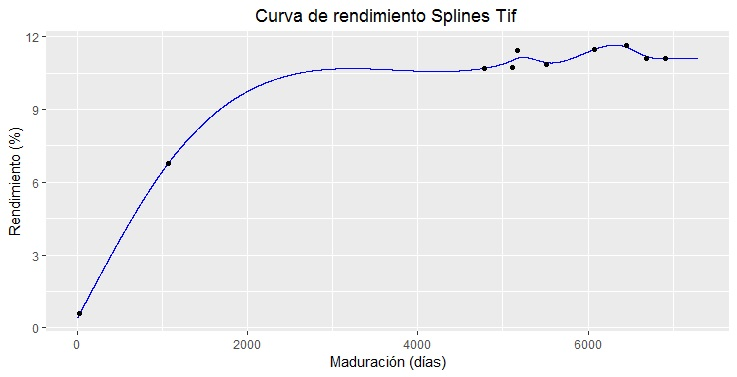
\includegraphics{images/c_tif.jpg}}
%\includegraphics[width=0.7\textwidth]{Imagen022.png}
\caption{Curva Spline TIF.}
\label{curva_spline_tif}
\end{figure}


\begin{figure}[h]
  \scalebox{0.80}{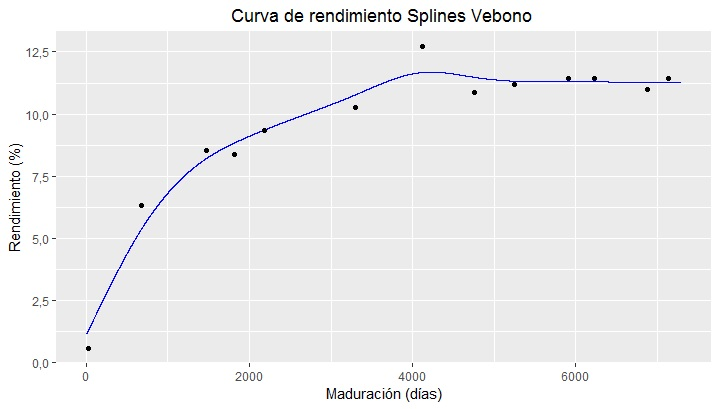
\includegraphics{images/c_veb.jpg}}
%\includegraphics[width=0.7\textwidth]{Imagen022.png}
\caption{Curva Spline VEBONO.}
\label{curva_spline_veb}
\end{figure}

\newpage

\subsection{Comparativo curvas de Rendimiento.}\hspace{5cm}

\hspace{0.4cm} En las figuras \ref{curva_spline_comp_tif} y \ref{curva_spline_comp_veb} , se muestra una comparaci\'on entre las curvas de rendimiento obtenidas mediante la metodolog\'ias de Splines de suavizado, Svensson sin opmitizar y Svensson Optimizado.
Para el caso de la metodolog\'ia de los Splines se us\'o un par\'ametro de suavizamiento de 0.2, el mismo controla la suavidad de la curva obtenida. Por su parte las curvas obtenidas para las metodolog\'ias de Svensson optimizada y sin optimizar surgen de los par\'ametros considerados al momento de calcular los precios te\'oricos de los instrumentos.

\hspace{0.4cm}Recordemos que para la metodolog\'ia Svensson sin optimizar se usaron unos par\'ametros por defecto, mientras que para la metodolog\'ia de Svensson optimizada se usaron aquellos par\'ametros de minimizaran la diferencia entre los precios te\'oricos y los precio promedio. 

\newpage

\begin{figure}[h]
  \scalebox{0.65}{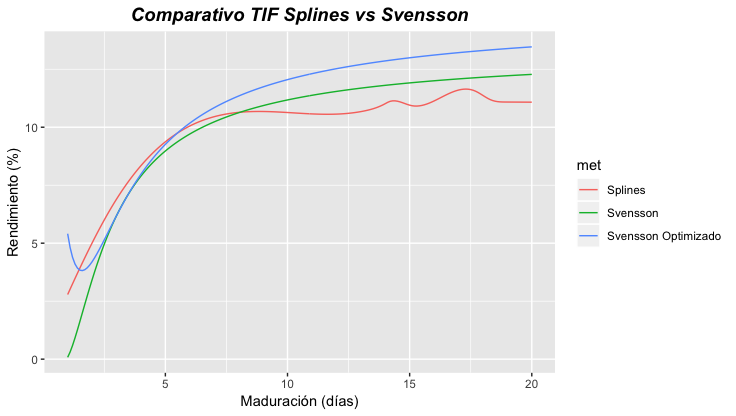
\includegraphics{images/Comparativo_tif.png}}
%\includegraphics[width=0.7\textwidth]{Imagen022.png}
\caption{Curva TIF Spline vs Svensson.}
\label{curva_spline_comp_tif}
\end{figure}


\begin{center}
{\begin{tabular}[t]{|c |c |c |c |c |c |c |c |r|}
\hline
Metodolog\'ia / Par\'ametro / TIF & $\beta_{0}$ & $\beta_{1}$ & $\beta_{2}$ & $\beta_{3}$  &  $\tau_{1}$ & $\tau_{2}$ \\
\hline
Svensson sin optimizar & 0,1337 & -0,0100 & -0,3078 & -0,1340  & 0,5453 & 0,3506\\
\hline
Svensson Optimizado & 0,1430 & 0,2119 & -0,6438 & 0,3327 & 0,5744 & 0,0184 \\
\hline
\end{tabular}}
\end{center}




\newpage

\begin{figure}[h]
  \scalebox{0.65}{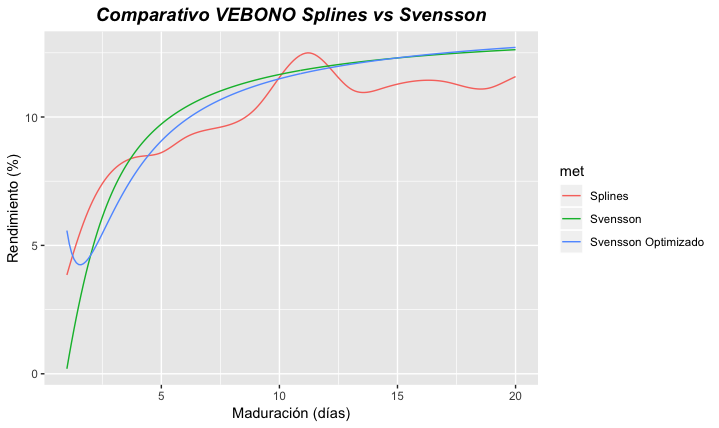
\includegraphics{images/Comparativo_vebono.png}}
%\includegraphics[width=0.7\textwidth]{Imagen022.png}
\caption{Curva VEBONO Spline vs Svensson.}
\label{curva_spline_comp_veb}
\end{figure}

\begin{center}
{\begin{tabular}[t]{|c |c |c |c |c |c |c |c |r|}
\hline
Metodolog\'ia / Par\'ametro / VEBONO & $\beta_{0}$ & $\beta_{1}$ & $\beta_{2}$ & $\beta_{3}$  &  $\tau_{1}$ & $\tau_{2}$ \\
\hline
Svensson sin optimizar & 0,1358 & 0,1000 & -0,5037 & -0,2887 & 0,1195 & 0,5017\\
\hline
Svensson Optimizado & 0,1421 & 0,4845 & -0,4343 & -0,3514 & 0,1985 & 0,7851 \\
\hline
\end{tabular}}
\end{center}


\newpage

\section{Conclusiones y Recomendaciones.}

\hspace{0.4cm}La curva de rendimiento es una herramienta muy importante al momento de obtener informaci\'on acerca de la tasa de inter\'es o rendimiento a una fecha determinada ya que dicha curva relaciona la maduraci\'on o fecha de vencimiento con el rendimiento. Una de las aplicaciones de esta curva, es que a partir de ella es posible obtener con facilidad el precio de un determinado instrumento, bono o t\'itulo, lo cual es de suma utilidad al momento de querer realizar alguna operaci\'on con el mismo, ya sea compra o venta del instrumento, ya que se tendr\'ia de antemano un precio referencial a partir del cual se puede tomar una decisi\'on. En otras palabras, la curva de rendimiento es una herramienta muy \'util al momento de tomar decisiones al realizar alguna inversi\'on.



\hspace{0.4cm} Para determinar dicha curva, varias metodolog\'ias han sido desarrolladas. Existen dos grandes enfoques que permiten su c\'alculo, el primer enfoque se basa en el uso de las metodolog\'ias param\'etricas de estimaci\'on, las cuales se caracterizan por estar atadas a ciertos par\'ametros, su uso es muy frecuete. Entre ellas, principalmente destacan la metodolog\'ia de Nelson y Siegel introducida en 1987 $[2]$, la metodolog\'ia de Svensson desarrollada en 1994 $[3]$, entre otras.


\hspace{0.4cm}Por otra parte, el segundo enfoque se centra en el uso de las metodolog\'ias no param\'etricas, las cuales se caracterizan por su flexibilidad ya que ellas no se encuentran atadas a ning\'un par\'ametro espec\'ifico sino que trabajan directamente con los datos suministrados. Entre ellas, destacan la metodolog\'ia de redes neuronales $[9]$, splines de polinomios $[6]$, splines c\'ubicos suavizados $[7]$, entre otras. En el presenta trabajo se aplica la \'ultima metodolog\'ia mencionada.


\hspace{0.4cm} La principal raz\'on de aplicar la metodolog\'ia de los splines c\'ubicos suavizados, fu\'e el balance que se obtiene como la misma, ya que ella presenta un equilibrio entre el ajuste a los datos y la suavidad de la curva resultante. Lo cual, es \'util cuando la data presenta mucho ruido ya que esta metodolog\'ia no interpola los valores ingresados sino que ajusta una curva suave que presenta el menor error de ajuste posible. En el presente trabajo se emple\'o la data de los Tif y Vebonos, instrumentos de la deuda p\'ublica nacional venezolana para el a\~no 2016 y 2017. Para ambos intrumentos se encontraron una cantidad aceptable de operaciones a partir de las cuales se calcu\'o el rendimiento y as\'i a partir de dichos valores calcular la curva de rendimientos. Una vez obtenida la curva, se procede a estimar los precios de los instrumentos involucrados.



\backmatter

\begin{thebibliography}{99}

\bibitem{Mm} {\sc Maita B. Miriam A.}, {\it Estimaci\'on de una curva de rendimientos para los bonos de la deuda p\'ublica interna en Venezuela}, (trabajo de grado Maestr\'ia en Administraci\'on de Empresas menci\'on Finanzas).  Universidad Cat\'olica Andr\'es Bello, Caracas, Venezuela, 2010.

\bibitem{NS} {\sc Nelson, C. y Siegel, A.} {\it Parsimonius Modeling of Yield Curves}. Journal of
Business, $60$: $473$-$489$, 1987.

\bibitem{DO} {\sc Douglas, L.G.} {\it Yield Curve Analysis}. New York Institute of Finance, 1988.


\bibitem{Sv} {\sc Svensson, L.} {\it Estimating and Interpreting Forward Interest Rates: Sweden 1992-1994}, NBER Working Papers, 4871. Estocolmo: National Bureau of Economic Research, 1994.

\bibitem{HT} Hunt, B. y Terry, C. {\it Zero-Coupon Yield Curve Estimation: A Principal Component-Polynomial Approach}, Technical report 81. Sydney: University of Technology Sydney - School of Finance and Economics, 1998.

\bibitem{NW} Nocedal, J. y Wright, S. {\it Numerical Optimization}. New York: Springer-Verlag, 1999.


\bibitem{FG} Fan, J. y Gijbels, I. {\it Local Polynomial Modelling and Its Applications}. New York: Chapman and Hall, 1996.

\bibitem{BW} B.W. Silverman. {\it Some Aspects of the Spline Smoothing Approach to Non-Parametric Regression Curve Fitting}. Journal of the Royal Statistical Society. Series B (Methodological), Vol. 47, No. 1, 1(1985), pp. 1-52, 1984.


\bibitem{F} Friedman, J. H. {\it A Variable Span Smoother}, Technical report 5. Standford:
Standford University - Departament of Statistics, 1984.


\bibitem{SH} Sharda, R. {\it Neural networks for the MS/OR analyst: An application bibliography}. Interfaces, 24(2): 116-130, 1994.

\bibitem{FR} Fern\'andez J.L., Robles, M.D.  {\it Teor\'ia de las Expectativas y Cambio Estructural: nueva evidencia en los tipos a corto plazo espa \~noles.} Tribuna de Econom\'ia No. 827. ICE, 2005.

\bibitem{YS} Yung-Shi Liau, Jack J.W. Yang. {\it The Expectations Hypothesis of Term Structure of Interest Rates in Taiwan's Money Market.} International Research Journal of Finance and Economics, 2009.

\end{thebibliography}



\end{document}
